\documentclass{phyasgn}\usepackage{nag}
\phyasgn{classname=挑战杯五四青年科学项目}
\usepackage{siunitx}
\usepackage{subfig}
%\ctexset{punct=kaiming}
\setCJKmainfont[ItalicFont=FZKTK.TTF,BoldFont=FZXBSK.TTF]{FZSSK.TTF}
\setCJKsansfont[BoldFont=FZHTK.TTF]{FZXH1K.TTF}
\setCJKmonofont[ItalicFont=FZKTK.TTF]{FZFSK.TTF}
\newCJKfontfamily\FZSS{FZSSK.TTF}
\newCJKfontfamily\FZKT{FZKTK.TTF}
\newCJKfontfamily\FZFS{FZFSK.TTF}
\newCJKfontfamily\FZHT{FZHTK.TTF}
\setmainfont{TeX Gyre Termes}
\setsansfont{TeX Gyre Heros}[Scale=MatchLowercase]
\setmonofont{Ubuntu Mono}%[Scale=MatchLowercase]
\newfontfamily\lm{Latin Modern Roman}
\usepackage{unicode-math}
\setmathfont{TeX Gyre Termes Math}
\newcommand\keywords[1]{\textbf{关键词}: #1}
\newcommand{\enabstractname}{Abstract}
\newenvironment{enabstract}{%
  \par\small
  \noindent\mbox{}\hfill{\bfseries \enabstractname}\hfill\mbox{}\par
  \vskip 1ex}{\par\vskip 1ex}
\newcommand\pkg[1]{\textsf{#1}}
\newenvironment{csop}{\vskip\topsep\noindent\hspace{2em}\ttfamily\small\ignorespaces}{\vskip\topsep\par}
\usepackage{float}
\usepackage{booktabs,metalogo,siunitx,marginnote,manfnt,url}
\usepackage[unicode]{hyperref}
\hypersetup{pdfstartview=XYZ,hidelinks,pdfcreator=XeTeX Output,pdfauthor=xxx,
pdftitle=抗议、镇压与宣传反制:来自哥伦比亚的证据}
\urlstyle{same} 
\usepackage{geometry,fancyhdr}
\geometry{left=3cm,right=3cm,marginparwidth=4em}
\fancyhead[L]
{\begin{tabular}[b]{@{}l@{}}
  \hyperref{https://www.pku.edu.cn/}{}{}{
\includegraphics[height=2.12em]{pkulogo.jpg}}
\end{tabular}}
\fancyhead[C]
{
  \large 
  抗议、镇压与宣传反制:来自哥伦比亚的证据
}

\usepackage{shortvrb,fancyvrb}
\MakeShortVerb|
\fvset{xleftmargin=2em,fontsize=\small}
\makeatletter
\ifx\l@nohyphenation\undefined
  \newlanguage\l@nohyphenation
\fi
\DeclareRobustCommand\meta[1]{%
  \ensuremath\langle
  \ifmmode \expandafter \nfss@text \fi
  {%
    \rmfamily\itshape
    \edef\meta@hyphen@restore
    {\hyphenchar\the\font\the\hyphenchar\font}%
  \hyphenchar\font\m@ne
  \language\l@nohyphenation
  #1\/%
  \meta@hyphen@restore
  }\ensuremath\rangle
}
\makeatother

\def\phyasgn{\pkg{phyasgn}}
\def\version{0.2 $\upbeta$}

\title{
  {抗议、镇压与宣传反制:来自哥伦比亚的证据}
}
\author{小组成员:张维翰\thanks{200001694
8@stu.pku.edu.cn,政府管理学院,公共管理类},邓晨钰\thanks{dengcheny
u11@126.com,外国语学院,西班牙语专业},范一苇\thanks{fyw233@outlook.com,外国语学院,西班牙语专业},姜雨玥\thanks{2100018504@stu.pku.edu.cn,外国语学院,西班牙语专业},邱文治\thanks{own@pku.edu.cn,历史学系,外国语言与外国历史专业},吴熙楠\thanks{xinanwu@pku.edu.cn,物理学院,物理专业}}
\date{\today}
\begin{document}
\maketitle
\begin{abstract}
2021年4月,哥伦比亚爆发了声势浩大的反税制改革游行示威活动,为平息这场社会动乱,政府采取妥协让步、信息控制、暴力镇压等综合的政治控制手段。但并非所有措施都取得成效,很多暴力治安手段甚至引起了更多的抗议以及冲突的升级。本小组利用数据处理、文本分析、线上访谈等研究方法对示威活动和政府应对措施进行考察,并将其作为样本探究政府面对社会抗议时的应对机制及其效果。
\end{abstract}
\keywords{抗议,镇压,政治控制,哥伦比亚,警察暴力,税制改革}
\vspace{6em}
\begin{enabstract}
In April 2021, Colombia witnessed a massive demonstration against the tax reform and the government used a combination of compromise, information control and violent repression to quell the social unrest. However, not all measures were effective, and many of the violent policing tactics even led to more protests and an escalation of the conflict. Using data processing, textual analysis, online interviews and other research methods, our group examines the demonstrations and government responses, and uses them as a sample to explore the government's coping mechanisms and their effectiveness in the face of social protest.
\end{enabstract}\vspace{0.5em}
\noindent
\textbf{Keywords:} Protest, Repression, Political Control, Colombia, Police Violence, Fiscal Reform
\clearpage
\tableofcontents
\clearpage
\section{导言}
十几年前,彼得·史密斯在《拉美的民主》曾通过调查得出一个令很多人惊讶的结论:“拉美大陆并不是一个能动主义的社会”(Smith, Peter H.2013)。也就是说,抗议游行在拉美已经不再是一个常见的事情了。但伴随着新自由主义的彻底失败,以及在世界经济不景气背景下贫富差距等社会问题进一步凸显,激化的社会矛盾让拉美的抗议活动频起,并且往往很暴力。二十一世纪的第二个十年,拉美很多国家都爆发了激烈的社会抗议运动。
\par 2021年4月28日,一场全国性的示威游行席卷了哥伦比亚。抗议者打出反对税制改革的旗号,要求政府撤回其刚刚通过的新税法,该法为了弥补疫情期间政府的财政损失,提高了个人所得税的征收范围,并且对很多日常用品、食品的商品税进行了调整——这意味着在疫情本身失业人口大大增加、个人收入减少的情况下,人们需要缴纳更多的税。恰逢五一劳动节,示威活动迅速发展,人们占领了街道。出现了多起警察和示威群众冲突事件,血腥暴力的视频图像材料充斥网络——在波哥大,在卡利,并不能确定是抗议者还是警察率先使用了暴力。即使政府很快就叫停了税制改革,物价也恢复了正常,抗议活动也依旧在继续——很显然抗议的目标已经由对税制改革的不满转移到了对长期以来的社会不平等以及国家深层次政治问题的抗争。《哥伦比亚社会抗议》的作者毛里西奥·阿基拉(Mauricio Archila)评价认为这场运动涉及范围之广、持续时间之长在哥伦比亚历史上都是前所未有的。几十年来第一次,哥伦比亚的各个社会阶层各种职业共同参与社会抗议,疫情造成的经济不景气造成哥伦比亚长期新自由主义经济政策的动摇,一向以强硬著称的总统权威也受到了广泛质疑。(Daniel Pardo, 2021)
\par 随着时间的推移,示威运动逐渐受到了控制。几个月后,除了少部分专门的抗议组织还在组织示威活动外,大多数哥伦比亚人的生活已经恢复了宁静。政府在几个月后重新提出了新的税制改革方案,虽然依旧出现了零星的抗议示威活动,但是总体而言在政府的解释宣传下,大多数人很快就接受。正如政治学家桑德拉·博尔达(Sandra Borda)在抗议开始阶段所预测的那样,政府采取了镇压和温水政策结合的方式,逐渐平息了这场社会动乱\footnote[1]{"Yo creo que vamos a ver una combinación de represión con pañitos de agua tibia"。}(Daniel Pardo, 2021)。而另一方面,正如在访谈中几乎所有人回答的那样:在激烈的示威之后,没有任何事情发生了改变。
\par 2021年哥伦比亚示威抗议爆发期间,本小组的成员就非常关注事态发展,并通过社交媒体和哥伦比亚的朋友了解该事件的发展状况,特别关注社交媒体上政府和民众在警察暴力等问题上的冲突:伴随示威运动发展,政府如何调整政策、采取措施来应对混乱和人们的诉求,而这些措施又对示威游行造成了什么样的影响。抱着这些问题,本小组同学充分发挥不同学科背景合作的优势,运用不同的研究方法,开展互补的、跨学科的学术训练。一方面,大量搜集来自哥伦比亚政府、世界银行等国际组织以及拉美晴雨表等权威机构的数据,并取得哥伦比亚反警察暴力非盈利组织Grita的帮助,综合网络词频的统计工作,利用量化方法探究示威运动的规模变化及其影响因素;另一方面对影响深远的两次税制改革原文文件进行细致的文本分析,了解改革内容及其对大众产生的影响,并通过对比考察政府前后的改变和妥协。除此以外,本小组通过各种渠道联系到数位来自哥伦比亚的志愿者接受我们的线上,其中包括哥伦比亚日前最活跃的抗议组织“第一线”的发言人。访谈工作促进了小组成员对哥伦比亚社会各方面的认识,并且从微观层面填补了叙事细节的空白,也让我们进一步提出一些问题和猜想。在写作结构上,本文将分为三个部分,在第一个部分我们会阐述观察到的现象,并利用数据和访谈解释问题的提出;在第二部分我们会从哥伦比亚暴力的政治文化、不平等的经济社会现状以及哥伦比亚保守的政治特点来介绍这次示威游行的背景;在第三部分我们将深入讨论政府在此次示威中采取的措施以及这些措施对示威活动产生的影响,并得出最终结论。
\section{问题的背景:暴力、贫穷和右翼传统}
\subsection{暴力的政治文化:波哥大事件、游击队和准军事主义}
这次示威抗议中,游击队是否参与组织对政府的抗议行为,是一个罗生门事件,而整个过程中出现的暴力行为,无论是来自示威群众还是警察,都屡见不鲜。在探讨哥伦比亚问题的时候,我们经常可以看到有学者讨论一个问题:哥伦比亚是否存在一个暴力的文化传统?“即使用拉丁美洲国家的标准,哥伦比亚也算是一个暴力的国家” (Juan F. Vargas* and Raul Caruso, 2014),在这个国家的历史中发生了太多暴力事件,在哥伦比亚独立的两百年中,如果将政府军和游击队、武装集团的冲突都视为内战的话,哥伦比亚基本上一直处在内战状态:独立之后1830年起自由党和保守党断断续续的内战,历时三年死伤无数的“千日战争”,1948年波哥大事件之后十年“暴力”时期,以及六十年代之后游击队、贩毒集团和政府的斗争。二十世纪初乌里韦总统强硬的手段沉重打击了游击队和贩毒集团的势力,缩小了其势力范围,但同时又增强了政府“准军事主义”(paramilitarismo)的特点,让国家暴力机关对平民采取暴力行动变得合理。
\par 在历史上,波哥大事件(El Bogotazo)对于哥伦比亚形成这种暴力的政治文化具有重要作用,在波哥大事件中,农民、工人、学生这些社会力量被动员了起来。
\par 1948年4月,第九届泛美会议在波哥大召开,美国力求在冷战初期加大对拉丁美洲国家的控制。4月9日下午约一点,维护下层民众利益,主张反美反帝国主义的自由党民众主义领导人盖坦在波哥大的街头被人枪杀。
\par 波哥大市的市民、工人、学生愤怒地走上街头,发动了起义,起义群众占领了政府军武器库,打开监狱大门,袭击了包括国会大厦在内的许多建筑,大火将整个波哥大城市夷为平地,以至于波哥大如今的城市规划和建筑风格都和过去产生了巨大的改变(Karen Estupiñán, 2020)。盖坦被杀的消息迅速传到了哥伦比亚各地,愤怒的农民在各地都进行了示威游行活动,他们造成的破坏与波哥大市民相比更甚。政府迅速派出部队,在三天血腥的镇压之后,起义被平定。在之后被称为“十年暴力”(La Violencia)的时期,前后有三十万人被杀,而这一时期产生的影响远远不止如此。大量的农民、学生工人在遭受镇压之后转移到农村,山区,他们中的很多人都加入了六十年代以来逐渐兴起的游击队。波哥大事件彻底分裂了哥伦比亚,也有人认为波哥大事件之后,哥伦比亚就一直处在内战状态。
\par 六十年代的哥伦比亚山区,游击队逐渐发展了起来,其中力量最强大的是哥伦比亚革命武装力量(F.A.R.C),民族解放军(ELN),四月十九日运动(M-19)等。在盖坦之死15年后,英国左翼历史学家霍布斯鲍姆认为城市的斗争已经结束了,很难出现一个人能够对城市市民进行有效的动员了。但是农村的情况却大为不同,出现了很多由共产主义组织控制的农村,“共产主义地区有武装、有组织、有纪律,在共同的行政、教育和法律体系中。……它们最大的优势在于其吸引力,由于他们明显的效率和协议的公平性,邻近的农民很容易被吸引;……它最大的弱点是……他们的政治视野完全在当地,他们仅仅集中在自己的地区,难以挑战更高层次的行政和经济活动”(Hobsbawm,1963)。在最兴盛的时候,大部分的农村地区都在游击队的控制之下,一直到2002年乌里韦上台,用强硬的手段与游击队开战,才大大缩小了游击队的生存空间。游击队的主要战略有两点:一是通过领土扩张,用较为分散的地区控制更多的地区,将对抗扩大到全国各地,二是将其主要力量集中在其经济、战略决定性区域(Cadavid,2011)。
\par 为了维持革命活动,哥伦比亚革命武装力量等组织在山区种植毒品、进行绑架、在毒品种植地征收“革命税”。而M-19运动则致力于城市的恐怖活动。这些行为都让哥伦比亚人民对游击队产生了很深的恐惧。在当时的环境下,甚至很多富人会雇佣保镖来护送自己的孩子上学。总体而言,游击队和政府的内战是一场难以解释的战争,“不仅因为它的长度和它背后的各种动机和原因,而且还因为合法和非法的多个团体不断变化的参与,它广泛的地理分布,它在每个地区的特殊性,无论是在农村还是城市,都是如此”(Bello, 2013)。2016年,时任哥伦比亚总统桑托斯和FARC达成和平协议,政府对游击队让步很多,这引起了很多人的不满。人们认为,游击队的威胁只是从上层社会中消失了,但是底层人民、很多山区和农村这些威胁依旧存在,很多人看来和平协定并没有真正改变什么\footnote[2]{AIRI访谈稿等。}。
\par 除了游击队,准军事主义在哥伦比亚的发展也值得注意。在全国各地出现了类似于哥伦比亚联合自卫力量(AUC)这样的右翼准军事组织,他们对游击队员采取了“错杀一千也不放过一个”的政策。准军事主义并非一开始就被哥伦比亚国家所接受,它实际上是一种国家的恐怖主义。乌里韦上台后,认可了准军事主义,并将其制度化。一些数据显示,在哥伦比亚,被政府或者准军事主义杀死并抛尸的人要比南锥体国家失踪的人数还要多。需要注意的是,比如在乌里韦政府时期,出现了大量的Falso Positivo,很多并非游击队的人被杀死。我们可以借助“国家安全学说”来解释这一现象。“(根据这一学说)国际共产主义出现于任何地方,任何地方都有潜在的游击队……社会冲突、政治反对派、对于思想的议论、意识形态和文化的不和谐都是全面的革命战争……总体的、一般的和绝对的战争的鲜明体现。”(Fitch, 1998)\footnote[3]{J.塞缪尔·费茨:《拉美的武装力量和民主》(J.Samuel Fitch The Armed Forces and Democracy in Latin America)约翰·霍普金斯大学出版社1998年版. 第106页。转引自董经胜. (2003). 拉美军人与政治:理论与范式的演进. Shi Xue Li Lun Yan Jiu, (3), 94-106. \url{https://doi.org/10.3969/j.issn.1004-0013.2003.03.013}。}这些准军事组织在政府的包容和支持下快速发展,渗透到各地各个结构,在大学里,左翼教授被暗杀,教师、学生、工人团体被驱逐被解散。因此,由于所谓共产主义和游击队的威胁,以及毒品战争的需要,哥伦比亚每年维持了极高的军事以及警察等机构支出,并且长时间的内战,也让警察和军人采取暴力行为的倾向大大提高,尽管这个国家的民主制度在五十年代之后没有像其他南美国家那样遭到破坏,但是暴力已经成为这个国家的政治文化。
\subsection{艰难生活:贫富差距和社会问题}
	\begin{figure}[!h]
	\centering
	
\includegraphics[width=.9\linewidth]{pic/1.png}
	\caption{哥伦比亚国家的主要问题:2007-2018\protect\footnotemark[4]}
	\label{fig:1}
	\end{figure}
    \footnotetext[4]{此处以及本章之后的图表如无特殊注释均引用自拉美晴雨表Colombia|LAPOP|Vanderbilt University,\url{https://www.vanderbilt.edu/lapop/colombia.php}。}
    \par 在2019年的拉美晴雨表统计中,哥伦比亚多数人认为冲突、经济和腐败是国家最严重的问题。对于大多数示威游行的人来说,他们并非持有共产主义的信仰,也并非游击队。哥伦比亚和智利一样,都在经受着新自由主义带来的巨大社会问题。这些社会问题在疫情时代,经济发展停滞的情况下很快被激化暴露出来。
    \begin{figure}[!h]
    	\centering
    	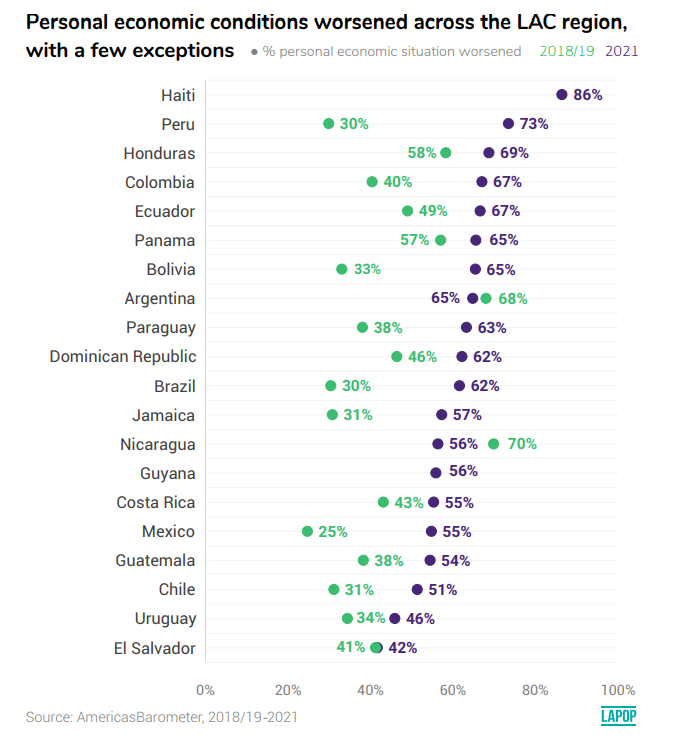
\includegraphics[width=.9\linewidth]{pic/2.png}
    	\caption{拉丁美洲各国疫情造成的经济衰退}
    	\label{fig:2}
    	\end{figure}
        \par 在分析这场由于税制改革引发的示威抗议运动时,我们必须先简单了解哥伦比亚当前社会的经济状况。2019年,即疫情爆发之前,有35.7\%——1750万人生活在贫困线下,在2014年到2019年五年间,底层40\%人口的财富增长率只有0.37\%,而基尼指数是0.513,这些数据都体现了哥伦比亚巨大的贫富差距\footnote[5]{世界银行数据,\\\quad
        \url{https://databank.worldbank.org/data/download/poverty/987B9C90-CB9F-4D93-AE8C-750588BF00QA/AM2020/Global_POVEQ_COL.pdf}。}。根据一些媒体2021年的报道,疫情发生后,贫困线下生活人数相比2019增长近7\%,达到42\%。而极端贫困人口则是达到了总人口的16\%。预估有2100万人每月可支配收入不到92美元,近200万人甚至无力确保自己的衣食住行,失业率增长5\%,达到19.5\%\footnote[6]{数据引用自Colombia VAM Bulletin,\\\quad
        \url{https://reliefweb.int/report/colombia/colombia-vam-bulletin-1-october-2021}。}。
        \par 在哥伦比亚,公民被分为六个等级,第一、二等级属于底层,第三、四等级属于中产阶级,第五、六等级属于富裕阶层。政府每年会进行调查统计,评定每个家庭的等级。一位受访者和我们描述了她所看到的情况:“穷人每天的收入在5000-45000比索左右,比如清洁女工,换算成月收入即15万到135万比索每月,年收入180-1620万比索。但是中产阶级(estrato 3-4)每月收入可以达到4000-5000万比索\footnote[7]{约合人民币6w9到8w6。}。作为参照的,政府公务员的工资在每月1800-2500万比索这样\footnote[8]{约合人民币三到四万。}。在很多沿海城市,如乔科市(Chocó)和瓜希拉市(Guajira),人民的生活水平都很差。在瓜希拉,土著社区甚至连饮用水和电力都没有,他们的土地经常被用来开采石油。农村的孩子每天要走3个小时的路来上课,但是在新冠疫情期间,因为他们没有网络,因此不能再网上上课。而在城市里,很多人都并没有自己的房子或者公寓,举一个最生动的例子,在波哥大,一个鸡蛋的价格是4000比索\footnote[9]{约合人民币7元。}。这也就是为什么当政府要人民再为基本的商品和食物供应缴纳19\%的税的时候,哥伦比亚人忍无可忍了。而对于一个没有全民医保的国家来说,如果没有EPS,你只有在等待两到三天之后才能得到医治,因此在疫情中很多人都死在候诊室里。”除此之外,虽然政府为适龄儿童提供了免费的义务教育,但只提供给最贫困的第一和第二等级,并且这种公立学校教师工资非常低,很难提供给学生有效的教学。而中产阶级和富裕的人们可以上私人学校,受访者Catalina Suarez所就读的Colombo American school,作为波哥大最好的几所中学之一,平均每年的学费达到2000万比索,这并不包括课外的补习费用以及准备ICFES(类似于中国高考)的费用,而2000万比索是很多家庭一年的全部收入。即使到了大学,学费依旧非常昂贵,在较好的大学,医学本科一个学期的学费可以达到2200万比索(三个月),除了政府提供了一小部分助学金奖学金外,贫困的孩子根本没有办法接触到高等教育\footnote[10]{参考AIRI访谈稿。}。
        \par 除了经济、教育、医疗方面的问题外,政府的腐败也是哥伦比亚社会所面临的重要问题。这严重影响了政府各个机构的威信。人们可能对政府本身很信任,但是政府中工作人员的腐败行为破坏了这一点。根据受访者的估计,每年政府机构腐败的金额可以达到50亿比索\footnote[11]{参见Camilo Mundólogo访谈稿:In Colombia, every year 5 billion pesos are stolen from the people and the government by ted officers. So when the government is running out of money, they just make up this kind of reforms and they want to get money from the common people.}。而且相比于其他国家,哥伦比亚对于腐败的刑法并不非常严格,在抗议示威发生后仅仅几个月,哥伦比亚科技部被曝严重腐败,原本应该用于农村地区无线网络建设的7000万比索被政府官员贪污。因此在2021年的抗议活动中,反腐败也是一个非常重要的口号。
        \begin{figure}[!h]
            	\centering
            	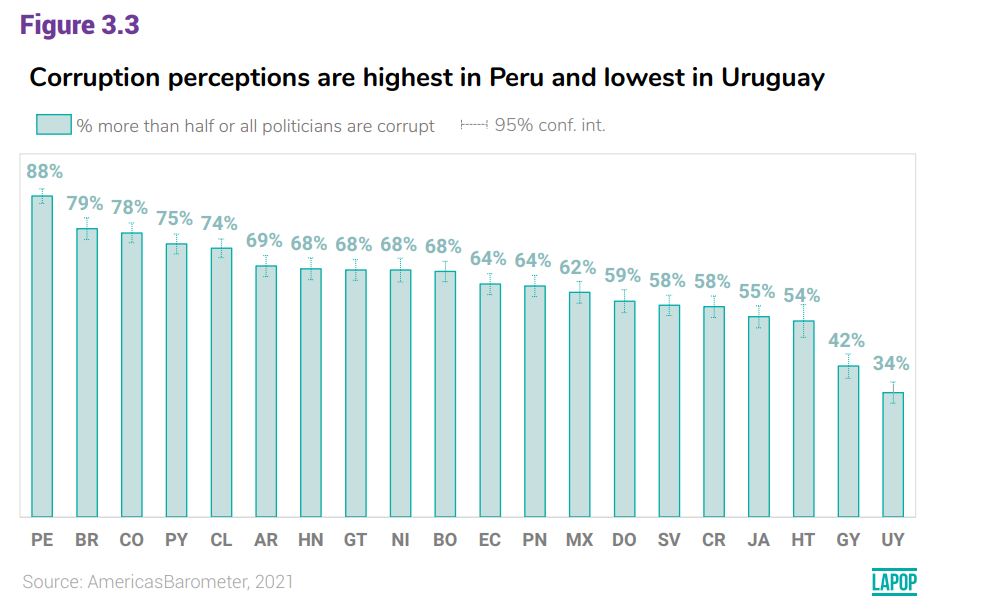
\includegraphics[width=.9\linewidth]{pic/3.png}
            	\caption{对出现腐败的预期(哥伦比亚高达78\%)}
            	\label{fig:3}
            	\end{figure}
    \subsection{保守和改变:右翼传统和大选展望}
    在历史上,哥伦比亚的政权几乎一直死死把握在右翼保守势力手中,甚至很多媒体将其称为“拥有200年右翼政府的国家”。这点是和其他拉美国家有很大不同的,其他拉美国家都曾出现的“钟摆效应”的现象并没有发生在哥伦比亚,即使是二十一世纪初,几乎所有其他拉美国家都是左翼掌权、查韦斯政府高举“二十一世纪社会主义”大旗的时候,哥伦比亚还在极右翼政客乌里韦的领导下利用各种残酷的手段追杀游击队。
    \par 独立之后,哥伦比亚的政治斗争主要发生在桑坦德派和玻利瓦尔派之间(自由党和保守党)。进入二十世纪之后,哥伦比亚出现了伟大的左翼民众主义政治家,自由派的领导人盖坦,他关心工人农民权益,主张要反对帝国主义对哥伦比亚的剥削,并且成功获得了自由党和部分保守党人士的支持。霍布斯鲍姆认为1930年以来在盖坦的领导下,哥伦比亚出现了一股社会主义的潮流,其意识形态更接近后来的菲德尔主义。哥伦比亚社会的政治精英不愿看到这样一位非常有个人魅力的左翼领导人上台,于是在1948年在波哥大街头枪杀了他。盖坦死后,哥伦比亚完成了自发的民众动员,但是在强大的反动保守政府的镇压下起义宣告失败。自那之后,哥伦比亚政治就继续被右翼保守的政治精英所控制,“全国阵线”之后,也有左翼政党的候选人曾经参与过总统大选,但几乎都以非常悬殊的差距输给右翼政治家。
    \par 但是这里的情况并非一成不变,正如之前所言,进入二十一世纪,一些左翼中左翼的力量开始出现在了政治舞台,并且在竞选中取得不错的成绩。2018年总统大选,来自人道哥伦比亚党的候选人,波哥大市市长古斯塔沃·佩特罗在第二轮大选中仅以微弱劣势输掉了大选。古斯塔沃·佩特罗曾是一名哥伦比亚武装游击队M-19运动的一员,该组织曾经策划过著名的司法大厦袭击等恐怖后动,因此佩特罗的游击队员身份在竞选阶段常常被他的对手批评,称呼其为恐怖分子。但是这些污名化行为并没有对其竞选产生特别大的影响。
    \begin{figure}[!h]
                	\centering
                	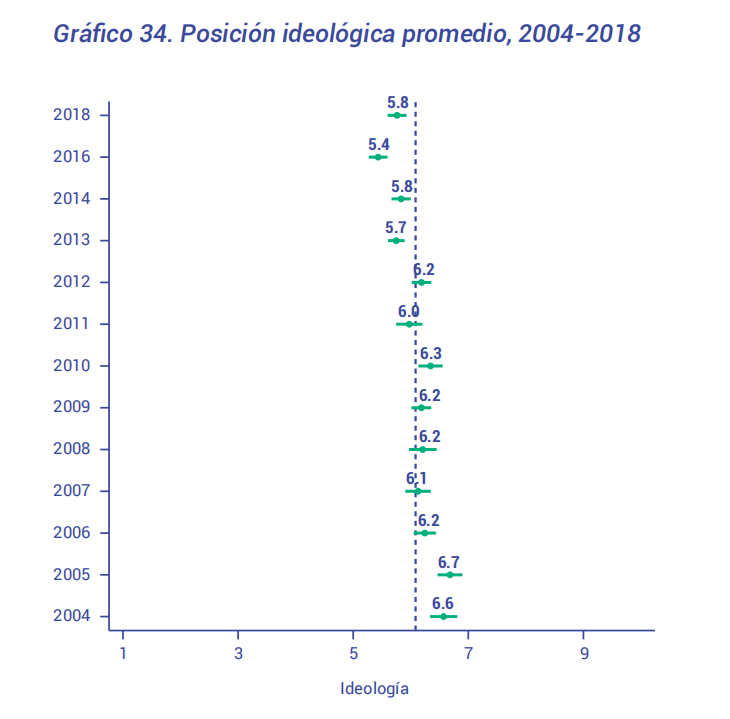
\includegraphics[width=.9\linewidth]{pic/4.png}
                	\caption{哥伦比亚意识形态中值定位,2004-2018}
                	\label{fig:4}
                	\end{figure}
    \par 2018年发布的美洲晴雨表显示,从2004年乌里韦的第一任任期到2018年杜克当选,哥伦比亚人民意识形态上的偏好出现了向左转的趋势。细究其中的原因,首先二十一世纪以来自由党和保守党两大传统政党快速衰落,更多政党出现在了哥伦比亚政治舞台。人们对政治的兴趣下降,也并不会将自己的想法归入某个党,这也给了新生的左翼政党和候选人以机会。其次长期新自由主义政策造成的巨大贫富差距,各种社会问题层出不穷,引起了下层民众的广泛抗议,长期的右翼执政也让人民感到厌倦,寻求“改变”的想法在群众间传播。再加上乌里韦采取强制的军事手段之后,游击队的力量大大下降,对于游击队的恐慌也不再如之前,左翼领导人开始在哥伦比亚政坛崭露头角。
    \begin{figure}[!h]
                    	\centering
                    	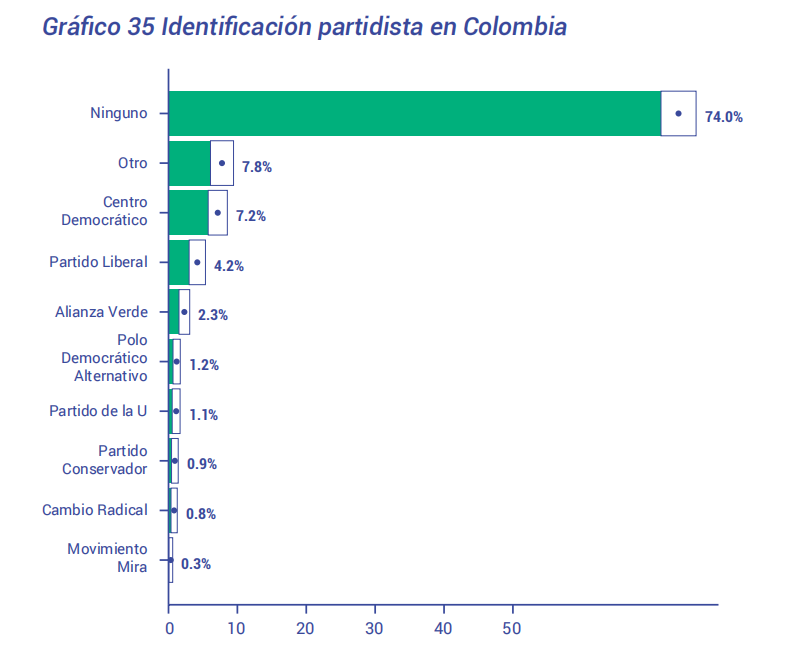
\includegraphics[width=.9\linewidth]{pic/5.png}
                    	\caption{哥伦比亚人民对各党派的认同}
                    	\label{fig:5}
                    	\end{figure}
\par 2022年5月,哥伦比亚大选又将如期举行,可以预见这将是非常值得期待的一次大选。首先,哥伦比亚的民主制度虽然从形式上比较稳固,但是哥伦比亚的人民也逐渐对其失去了信心。拉美晴雨表的调查结果显示,哥伦比亚只有26\%的人对民主制度感到满意,而相信选举的只有22\%的人。Camilo Mundólogo在接受访谈时说:“今年的选举非常重要,因为一方面,人们每天都对哥伦比亚以及邻国发生的事情感到越来越不舒服,这是一个严峻的形势。另一方面,在哥伦比亚及其边境地区,过去20年真的很困难,二十世纪我们可能可以达到真民主,而今天民主已经不再是真正的民主了。现在有其他的力量,不仅仅是人民或机构,还有机构背后操纵人民的黑暗力量。所以现在这次选举中要决定的事情真的很微妙。”\footnote[12]{参见Camilo Mundólogo访谈稿:“The election this year is very important because in one hand you have the people more and more uncomfortable everyday with what is going on not only in Colombia but also in the neighboring countries which is a critical situation. On the other hand, inside Colombia and its borders, the last 20 years have been really difficult because the democracy has turned into some kind of not really a democracy what probably could be in the 20th century. But now there’re other powers, not only the people or the institutions and the dark power behind the institutions that manipulates people. So right now the things to be decided in this election are really delicate.”}
 \begin{figure}[!h]
                    	\centering
                    	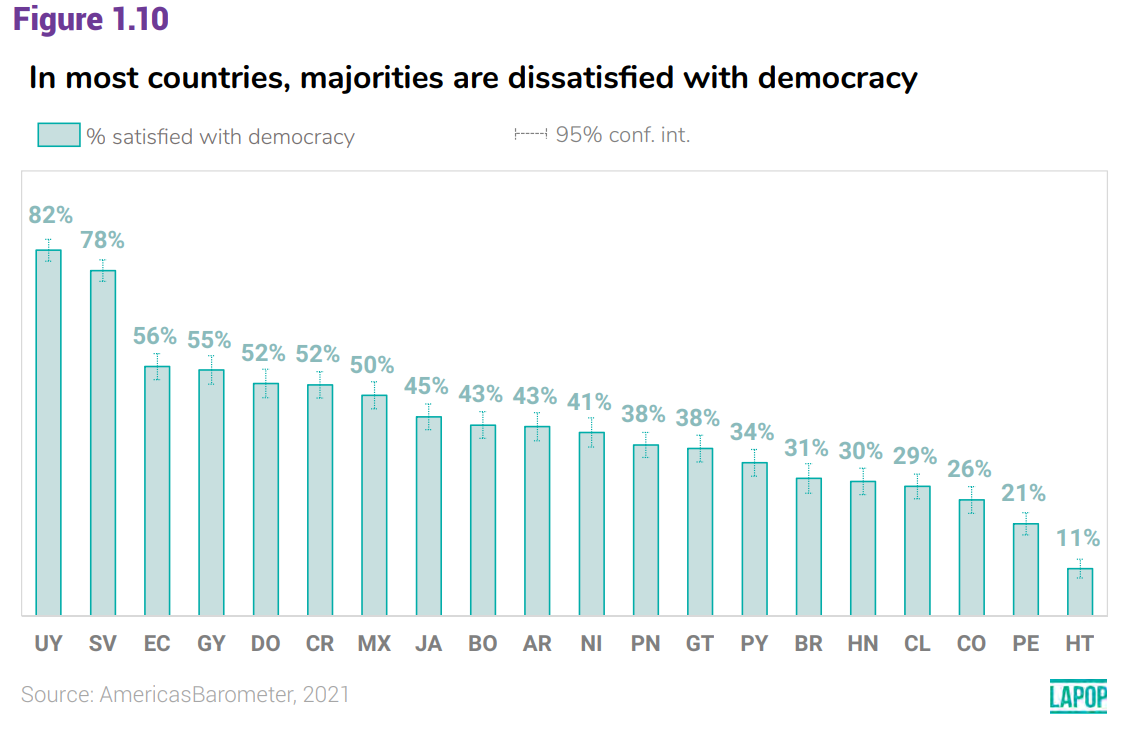
\includegraphics[width=.9\linewidth]{pic/6.png}
                    	\caption{哥伦比亚对民主的满意度只有26\%}
                    	\label{fig:6}
                    	\end{figure}
 \begin{figure}[!h]
                    	\centering
                    	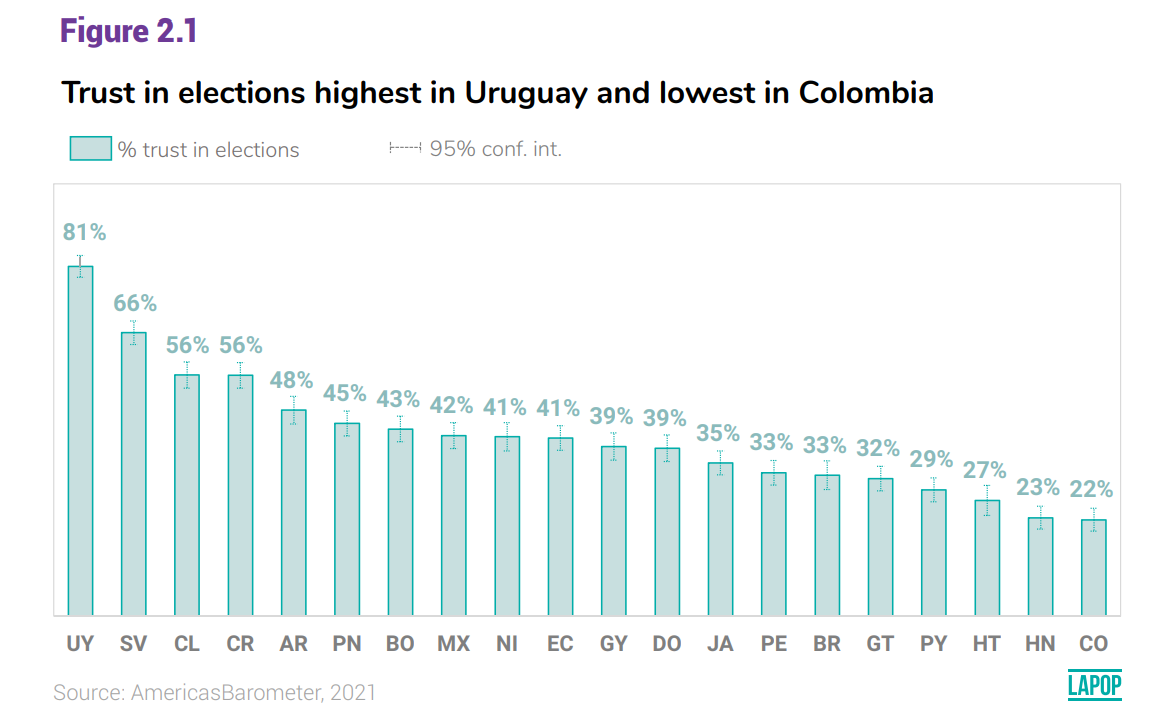
\includegraphics[width=.9\linewidth]{pic/7.png}
                    	\caption{哥伦比亚对选举的信任比例为22\%,是数据各国中最低的}
                    	\label{fig:7}
                    	\end{figure}
\par 更加值得注意的是,随着2021年智利和秘鲁大选左翼的胜利,拉美看起来再次迎来左翼集体上台执政。那么在这次所谓的“粉红浪潮”中,哥伦比亚的大选结果就非常令人期待。相比2018年第一次参加总统选举,这次古斯塔沃·佩特罗更加注意和一些右翼团体联合,这显然是为了赢得选举而进行的非常务实的行为,这也确实为他赢得了支持率。
\section{问题的探究}
\subsection{量化改革计划对抗议的影响}
\subsubsection{数据与方法}
为了量化改革计划对抗议的影响,我们利用了ACLED,即\textit{Armed Conflict Location \& Event Data Project}(Raleigh, Linke, Hegre and Karlsen 2010)。ACLED包含了全世界范围内关于政治暴力/抗议的事件级别的数据,如地点、日期、参与者、伤亡等。我们利用了2020年8月2日至2021年8月2日的数据,这段时间内的数据包括了全国范围内2150个抗议的观测值。
\par 我们的分析包括解释为什么4月28日国会通过法案可以看作随机的事件,以及如何使用时间断点回归 (Regression Discontinuity in Time) 来估计改革计划宣布前后抗议数的变化。在时间断点回归设计中,如果事件发生的时间点不是随机的,则会存在预期效应(Anticipation Effect),我们需要对此进行解释;同时我们还需要说明4月28日通过法案不是一个根据抗议的趋势而谋划的事件 (Hausman and Rapson, 2018)。我们使用了Google Trend来检测舆情的变化和公众的感知,从图中可看出,在4月28日国会通过法案前“改革”的搜索热度虽然有所上升但并不高,而在这之后才开始飙升,因而大部分公众并没有关心这项改革计划;同样地,如图,4月28日前抗议的总体趋势很稳定,国会通过法案的时间也并非有意为之。依据上述结论,断点回归在接近随机的断点处估计局部因果效应,从而能够很好地近似随机对照试验中的处理效应 (Wing and Cook 2013)。在这个断点回归设计中,我们使用的“驱动变量”为时间——在4月28日全国性大规模抗议爆发之前的日期取负值,之后的日期取正值。我们将4月28日设为断点(此处的驱动变量取值为0),这正好是哥伦比亚全国爆发大规模抗议的第一天。如前文所述,尽管改革计划早已于15日颁布,但直到28日改革法令在国会通过,改革的信息才广泛传播,随之抗议在全国范围内爆发,引起了广泛的媒体关注。依据 Cattaneo, Idrobo, and Titiunik (2020) 和 Gelman and Imbens (2019) 给出的建议,我们的局部多项式回归模型的阶数为2,这样能较好地反应数据的趋势又不会出现严重的过拟合现象。此外我们使用了三角核估计法 (Triangular Kernel) 以实现最优点估计。最后,我们使用标准的非参数方法选择最优带宽,这能够最小化局部多项式断点回归的点估计的均方误差 (mean-squared-error)。
\begin{figure}[!h]
                    	\centering
                    	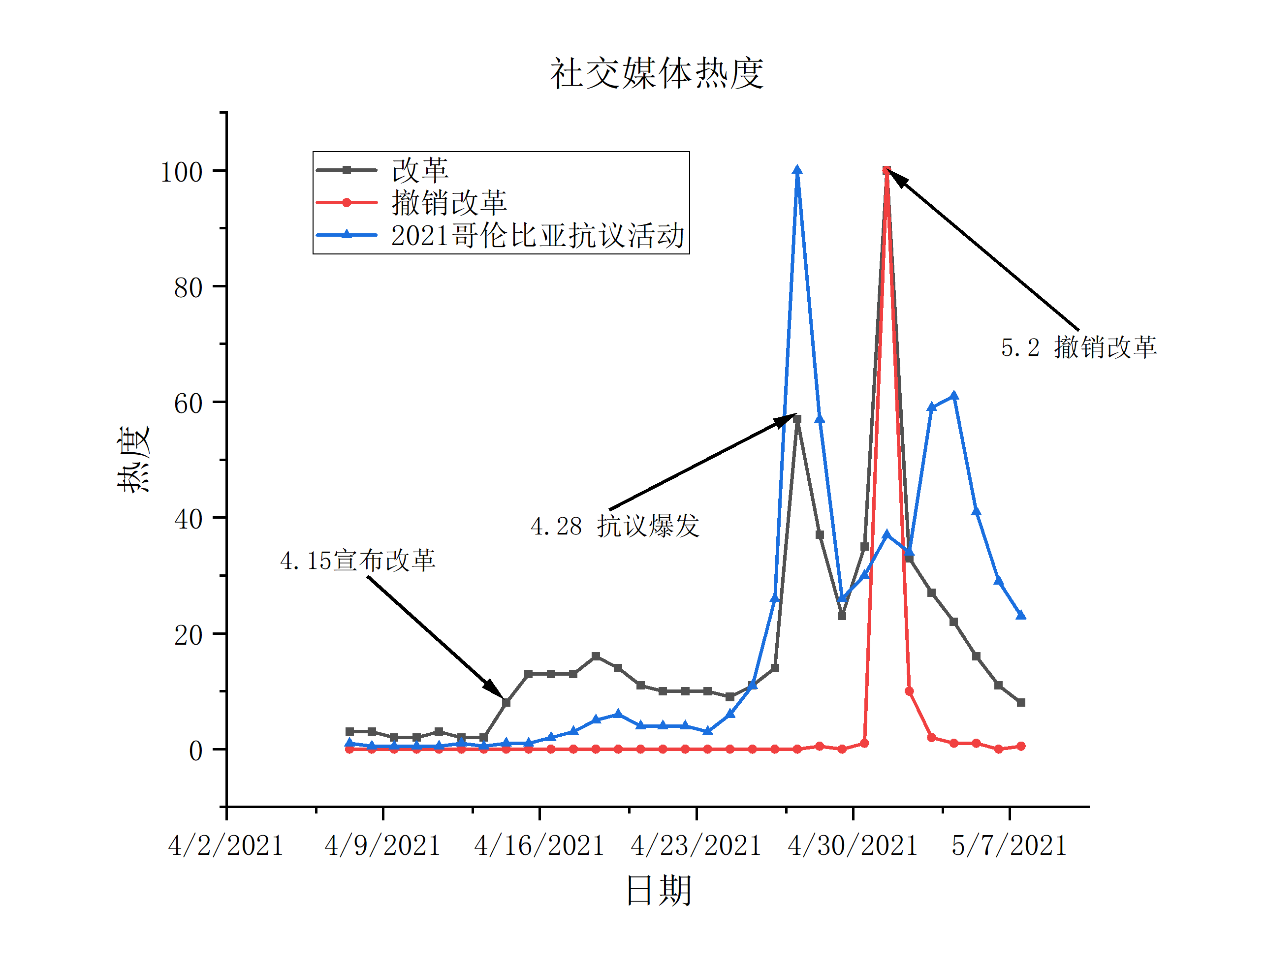
\includegraphics[width=.9\linewidth]{pic/8.png}
                    	\caption{哥伦比亚社交媒体热度随日期变化关系}
                    	\label{fig:8}
                    	\end{figure}
\subsubsection{结果}
如图所示,改革对抗议活动有着实质性的影响:在整个样本中,这次事件使得全国范围 内的抗议活动在断点周围平均每日增加了 65.82 次 (p < 0.001)\footnote[13]{使用Calonico, Cattaneo, Farrell and Titiunik 2017开发的stata工具包rdrobust, rdplot以及rdbwselect。}。误差修正后的断点回归结果呈现在表X里。虽然抗议数的增加十分迅速并且有着实质性意义,但数据告诉我们之后抗议数很快下降到之前的水平。改革后的抗议并没有维持在高水平(使用非参数方法估计时,在右侧临界点出现回升是因为过拟合,不能很好地预测之后抗议的趋势),说明有一些因素影响了抗议者的动机和行为,这激起了我们的兴趣。在接下来的章节里我们将详细讨论背后可能的原因。
\begin{figure}[!h]
                    	\centering
                    	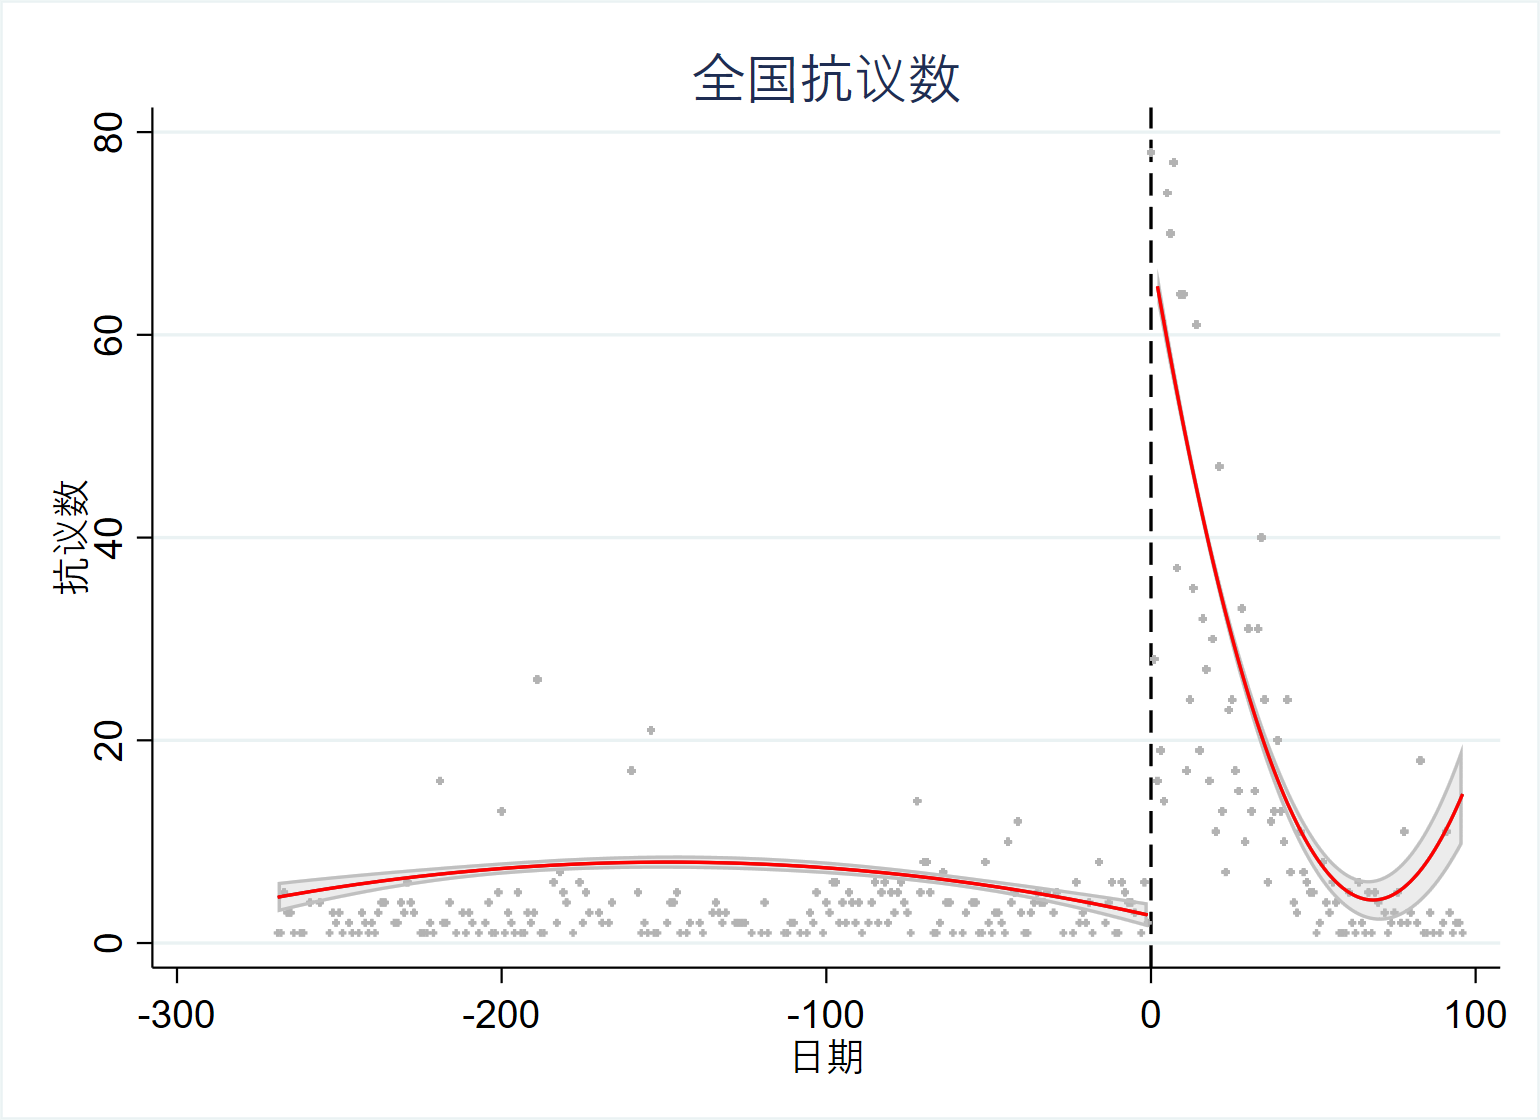
\includegraphics[width=.9\linewidth]{pic/9.png}
                    	\caption{哥伦比亚全国抗议数随日期变化}
                    	\label{fig:9}
                    	\end{figure}
\begin{figure}[!h]
                    	\centering
                    	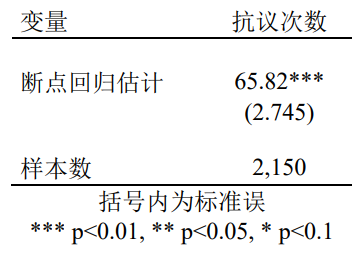
\includegraphics[width=.6\linewidth]{pic/10.png}
                    	\end{figure}
\subsubsection{稳定性检验}
在时间断点回归里,我们无法直接检验是否存在人为干预断点两端样本随机分配的情况 (Hausman and Rapson, 2018),如前文所述,我们可以大致认为处理是随机的并且不存在预期效应。依据Hausman and Rapson (2018)的建议,我们还进行了如下的检测:(1)断点敏感性检验,我们调整断点位置后,发现结果要么不显著、要么系数为负,说明断点的选择无误;(2)带宽敏感性检验,同样地调整带宽后,结果依然稳健;(3)平稳性检验,鉴于时间序列数据的特征,我们使用Dickey–Fuller Test (Dickey and Fuller, 1979)检验处理前(即4月27日之前)的数据,得到平稳的结果,说明在此之前抗议数没有明显的趋势。
\subsection{访谈方法:把握抗议全景}
除了搜集相关数据并进行处理,我们还通过访谈的方式,以了解数据无法涉及的领域,窥得这次抗议和镇压事件的全景,并且进一步完善研究的问题意识,补充叙事的缺失。
\par 在可获得性、接近性的基础上,我们在访谈对象选择上尽量追求其典型性。我们访谈了哥伦比亚近年来最为活跃、最有影响力的抗议示威组织“La Primera Línea”波哥大组织的发言人,获取来自抗议参与者和组织者的声音;我们联系了警察暴力统计机构Grita,就一些数据上得到他们的帮助。除此以外,我们的访谈对象从家境良好的Cornell大学博士到贫困线以下的小学教师,从旅居中国的中年作家到在阿根廷上学的大学女生,有得过新冠关心底层群众的波哥大高中生,也有积极参与抗议活动的地区青年。在我们选取访谈对象的过程中,最为遗憾的是并没有能够联系到一些知识水平较低的人,特别是农民、工人等集体,这也给我们访谈的成果带来了很大的局限性。
\par 在访谈提纲的设计上,我们并没有把问题局限于2021年的抗议活动,而是扩展到哥伦比亚生活、政治等方面。这是因为我们对于哥伦比亚仅仅局限于书面,对于哥伦比亚社会的各种具体情况缺乏了解,很容易对很多概念没有正确的认识,不利于我们在研究中提出恰当的问题。比如我们在访谈中具体询问了在生活中他们对于收入、物价的概念,并请受访者进行了举例,这样我们更容易理解2021年4月税制改革方案中增值税的提高对人们生活的影响。我们还针对不同的人设计了不同的访谈提纲,比如针对学生,我们会问一些关于教育、学费、日常生活这些问题,而对于抗议组织和一些对政治非常关心的人,我们会详细了解他们对于哥伦比亚政治的态度。通过这样比较有独特性的访谈,我们了解到不同的人对“是否有游击队、武装组织参与了抗议”以及“警察暴力和示威群众暴力是否有先后关系”这些问题有着不同的认识,进而提出了本论文的一些问题和论点。
\section{问题的讨论:哥伦比亚政府对抗议的反应及效果}
\subsection{理论框架}
顺利推行政策、维护国家的运转是各政体的执政者所面临的共同话题。为获得社会的支持和服从,并减少执政过程中的阻力和反抗,政府往往会同时采取一系列综合性手段,包括暴力及非暴力的镇压(repression),教化(indoctrination),以及福利措施(welfare programs)和引诱(inducement)等。这些看似不同的手段都是为了减少执政时的阻力,而为了更好地达成这一目的,在某些情况下各类策略也会互相补足。政治控制(political control)的概念可以将这一系列综合策略纳入到同一框架之中:策略的本质目标不变,只是在表现形式上有暴力程度、可感知程度等方面的区别。(Hassan et al., 2022)需要注意的是,政治控制手段并不总是能达到压制反对意见和政策推行阻力的目标。在部分情况下,镇压等手段反而会激起抗议的“反噬”(backfires),使得抗议在暴力程度上产生一定程度的升级(Ives \& Lewis, 2020; Odabaş \& Reynolds-Stenson, 2018; Earl \& Soule, 2010)。
\par 自2021年4月28日哥伦比亚全国抗议游行示威爆发起,哥伦比亚政府同样在全国各地综合采取了一系列政治控制手段,以达到减少抗议、推行税制改革的目的。根据暴力程度由低到高的顺序,首先,在税制改革的内容上,哥伦比亚政府做出了一定的让步,作为一种对最初抵制税制改革的反对人士的回馈(reward)或引诱。其次,哥伦比亚政府采取了一系列信息操纵(information manipulation)手段,包括在宣传上对抗议进行污名化、突出游行示威者的暴力举动,以及通过断电、打断拍摄、威胁拍摄者等方式阻止对政府不利的信息在各类媒体上的传播。最后,对游行示威的暴力镇压也是哥伦比亚政府采取的政治控制手段之一。然而,由警察和ESMAD进行的暴力镇压反而激发了抗议的进一步升级。通过对这一类反噬的机制分析,我们可以发现,哥伦比亚政府采取的其他政治控制手段可能有助于减少这类反噬,从而使得镇压达到最初的压制示威游行的目的。
\subsection{作为回馈和引诱的政策让步}
\subsubsection{两次改革整体框架对比}
\textbf{(1)四月税制改革的背景、内容及效果}
\par 2021年4月28日,哥伦比亚国会推出了总统伊万·杜克任期内的第三次税收改革方案《可持续团结法案》(Ley de Solidaridad Sostenible)。该方案旨在通过调节税收,应对由新冠疫情带来的财政和社会危机。当时哥伦比亚也正在经历来自委内瑞拉的移民潮危机\footnote[14]{参见Camilo Mundólogo访谈稿:“The government is broken because of the COVID-19, the Venezuela migration crisis and other things."},政府着力解决失业率飙升、国家财政恶化等紧急状况。此次改革的主要目的在于优化经济政策,以便在可持续的公共财政框架内巩固公平的基础设施、加强消除贫困的政策。
\par 改革方案共分为四编,第一编主要定义了财政规则的各项参数,规范了自治财政规则委员会的成员组成、职能范围与行使职权的方式,并对此前的部分同类法规做了修改和增订。第二编提出了团结收入计划,这是一项旨在促进减少贫困和缩小国内收入差异的永久性方案,相当于直接和定期的无条件货币转移;此外,特别提及关于促进就业的方案和对创造新的就业机会的奖励,以抵消新冠疫情带来的失业率上升,并提出总统拥有调整、重新安排行政和经济实体并对预算进行修改的特权。第三编分为两个部分,第一部分着重关注税收负担再分配的公平性,其中新增了针对普遍情况的“临时团结财富税”和针对月收入或进账超过 1000 万比索的个人的“临时高收入团结税”,将其规定为所得税的补充税种;第二部分侧重环境负担再分配的公平性,新增对于一次性塑料包装的国家性税收、农药的国家消费税和国家车辆税,规定首府城市可在取得市或区议会授权的前提下对所管辖的道路收费。第四编主要规定了增加收入和资源的预算措施,特别提出对老年人的国家社会保护计划捐款应在社会繁荣行政部内进行预算。
\par 5月2日,也即公布4天后,此次税收改革就因哥伦比亚全国上下数量激增的抗议示威行动而被迫终止。受访者在提及此次税收改革时,普遍表示改革会对国家的中下层阶级造成负面影响,对于在疫情期间已经持续恶化的国家经济无异于雪上加霜\footnote[15]{参见La Primera Línea采访稿。}。若改革得以实行,就连一枚鸡蛋的价格也将从1400比索涨到了2300比索\footnote[16]{参见Airi访谈稿:“I am very clear the one of eggs because of a first one egg, like in a very casual convenient store, it was like 1,400 pesos and after the tax thing, it increased to almost 2,300 pesos.”}。然而,正如背景中所述,哥伦比亚是一个贫富差异极大的国家,2021年最低工资约为245.09美元(Salario Mínimo Colombia, 2021),而据2021年5月2日前后的汇率计算,此次税收改革将个人所得税的起征点调整至月收入656美元。因此,这次税收改革将绝大部分哥伦比亚人都变成了纳税人,而其中有许多人仅能勉强养家糊口。物价的上涨远超近年来最低工资的提高,给农业生产带来了巨大挑战,因为农业的生产成本大幅增加,农牧产品的价格却几乎没有上涨,其他行业中刚起步的小公司也面临破产的风险\footnote[17]{参见Julieth采访稿。}。与此同时,在哥伦比亚每年都有50亿比索被政府官员贪污,政府缺钱时只会不断向穷人征税\footnote[18]{参见Camilo Mundólogo访谈稿:“In Colombia, every year 5 billion pesos are stolen from the people and the government by corrupted officers. So when the government is running out of money, they just make up this kind of reforms and they want to get money from the common people.”}。此次改革传递出一个在部分人看来很危险的信号:政府意在消除中产阶级、加剧贫富两极分化,尤其是诸如《可持续团结法案》等社会投资计划并没有真正帮助穷人\footnote[19]{详见William Andres Betancourt Villota访谈稿。}。但也出现了一些不同的声音:如一名受访者认为这次税收改革的误区在于向受到新冠疫情影响最大的中产阶级征收更多赋税,但总体来说国家确实需要更多税收来源,主要在于为长年没有支付应缴税额的大型企业破除特权豁免\footnote[20]{参见Jose访谈稿:“Maybe there was something like that it was really bad is that they wanted to be, I mean they warn the taxes were not going primarily to the rich people, they were going more to the middle class. Maybe this was a really bad decision, because I mean the middle class was one of the ones that had the highest impact because of COVID. So it was bad because of that. But I think that we need more taxes...We have to make exceptions some taxes exceptions so that these businesses can come here and build ourselves. The problem is that 20 years after they are not paying, I mean they pay tax but little tax.”应当指出,这位受访者的家庭条件较为富裕。}。总体来说,对于哥伦比亚广大中下层阶级来说,他们本就支付不起高昂的生活花费,更无力负担新增的各项繁杂税收,于是不得已中断工作生活走上街头抗议。作为回应,杜克政府撤销了这份草案,并在2021年7月推出了一项新的税收改革方案《社会投资法案》,最终该方案于9月得以通过并在2022年正式生效。
\par \textbf{(2)七月税制改革的内容}
\par 七月份的税收改革主要目的在于使各项财政政策能够以一种衔接紧密的方式运作,加强社会支出,促进经济复苏,创造就业机会和国家的财政稳定,维护商业结构,加强公共财政的可信度,以及避免最弱势群体的贫困加剧。此份草案相比四月份的草案更为简短,以财政政策措施和预算措施为总方法,共分为六章。第一章定义了税收正常化和对所得税的补充,介绍了一些程序性规则,并对所得税相关法规进行了修改。第二章明确了反逃税机制,修改了此前部分规定,和四月份的草案一样注明以电子发票的方式确定所得税和附加税税额。第三章侧重于紧缩部分开支和提高效率的措施,减少了国家预算中部分商品和费用的开支,依然保留四月份的草案中赋予总统的特别权力。第四章旨在加强社会支出和经济复苏,定义了团结收入计划和其他经济复苏措施,规定了增值税(IVA)的豁免商品名单。第五章介绍了作为公共财政可持续性机制的财政规则,修正了此前的法规。第六章提出将2021年度国家总预算增加140万比索,并将支出预算增加到147亿比索。
\par 总体上看,七月份税收草案(以下简称税收草案二)的第五章大致对应四月份税收草案(以下简称税收草案一)的第一编部分内容,只在顺序上做了调整。税收草案一的团结收入计划、支出方面的紧缩和效率措施也得到了保留,但税收草案二删去了关于临时团结财富税和临时高收入团结税的条款。在增值税(IVA)方面,税收草案二保留了部分免征税款的商品和服务名录。税收草案一中关于环境负担再分配公平性的条款基本被删去,车用汽油和ACPM附加费的相关条例也没有保留。针对第二份税收改革草案,受访者普遍表示比前一份更完善、更关注穷人的生计\footnote[21]{参见William Andres Betancourt Villota访谈稿:“I’m not really sure about that but I think that it was because that some senators tried to modify some things to make lives of poor people better.”},但对其具体内容不甚了解。
\par 税收草案二在交由国会讨论时,有15条被修订,其中包括:第18条,扩大团结收入的可能性,与其他社会计划衔接并重点关注女性照顾者;第22条,给予女性员工占最低月工资15\%的额外奖励,扩大国家政府激励创造新就业岗位的权力范围;第23条,要求招收第1、2、3等级\footnote[22]{哥伦比亚的家庭按经济状况从差到好分为1-6等级,1-3等级处于社会中下层。}家庭的孩子入学;第31条,将妇女和共和国国会经济事务委员会主席的参与纳入自治财政规则委员会。(Portafolio, 2021)这些修订反映出政府试图在保护妇女和其他弱势群体、扩大受教育权、促进就业等方面做出努力,以此贴近社会底层人民,对抗议者的诉求做出初步回应。接下来将对两份税收草案的具体条文和数据进行对比分析,探讨政府在税收草案二中做出的妥协与让步。
\subsubsection{征收目标调整的整体思路:从扩大税基到“开源节流”}
\begin{figure}[!h]
	\centering
	\vspace{-0.3\baselineskip}
	\subfloat{
		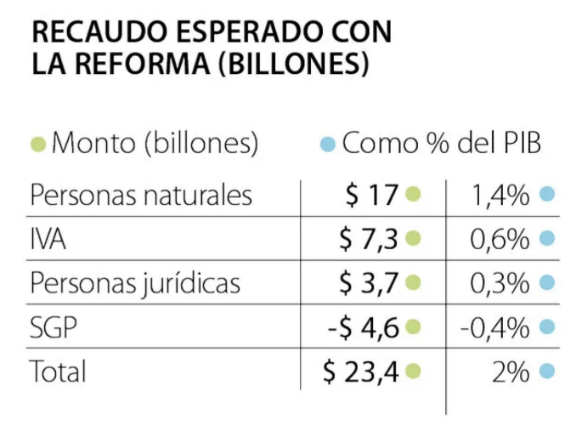
\includegraphics[width=.45\linewidth]{pic/11.png}}
	\quad
	\subfloat{
		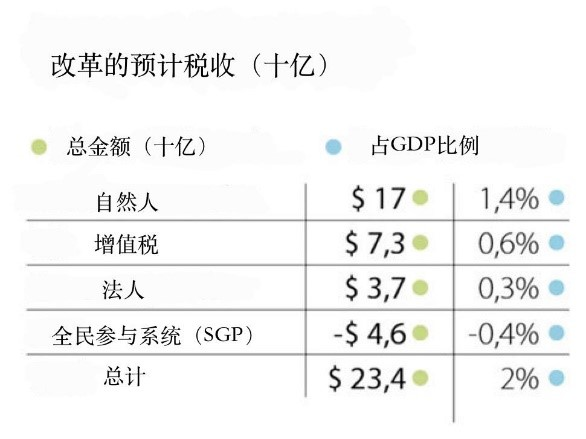
\includegraphics[width=.45\linewidth]{pic/12.jpg}}\\
	\caption{2021年4月税制改革的预计征收目标,图表来源\footnotesize{\url{https://www.larepublica.co/economia/cambios-en-el-iva-y-el-impuesto-de-renta-entre-los-aciertos-de-la-tributaria-para-anif-3158558}},数据来源:哥伦比亚财政与公共信贷部(Minhacienda),制图:LR-GR
}
	\end{figure}
    \par 在税收草案一中,哥伦比亚财政部预计将实现 234 亿比索的税收,其中 73 亿比索将通过增值税征收,170 亿比索将通过个人所得税征收,37 亿比索将通过法人所得税征收,。而46 亿比索将通过全民参与系统 (SGP)\footnote[23]{“全民参与系统(SGP, el Sistema General de Participación)”,于2001年建立,旨在将国家资源分配给地方,主要用于教育、卫生服务与社会保障。参见\url{https://www.mineducacion.gov.co/1621/articles-198471_archivo_pdf10.pdf}}分配到地方,用于教育、卫生服务和社会保障等领域,其中,就业促进、学费补贴和教育推广等项目将耗资8亿比索,另有18亿比索将用于支付增值税补偿\footnote[24]{增值税补偿(compensación del IVA), 指在一个给定的纳税期(通常是一个季度)内,进项税额高过销项税额,在这种情况下,如果纳税人按季度申报,则可以在随后的季度向财政部门要求退款或补偿。}。
\begin{figure}[!h]
	\centering
	\vspace{-0.3\baselineskip}
	\subfloat{
		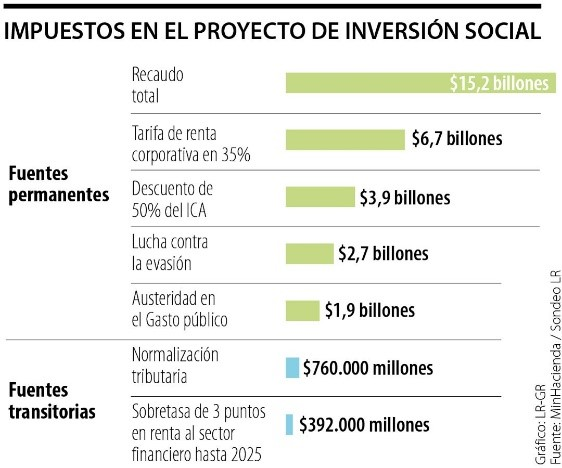
\includegraphics[width=.45\linewidth]{pic/13.jpg}}
	\quad
	\subfloat{
		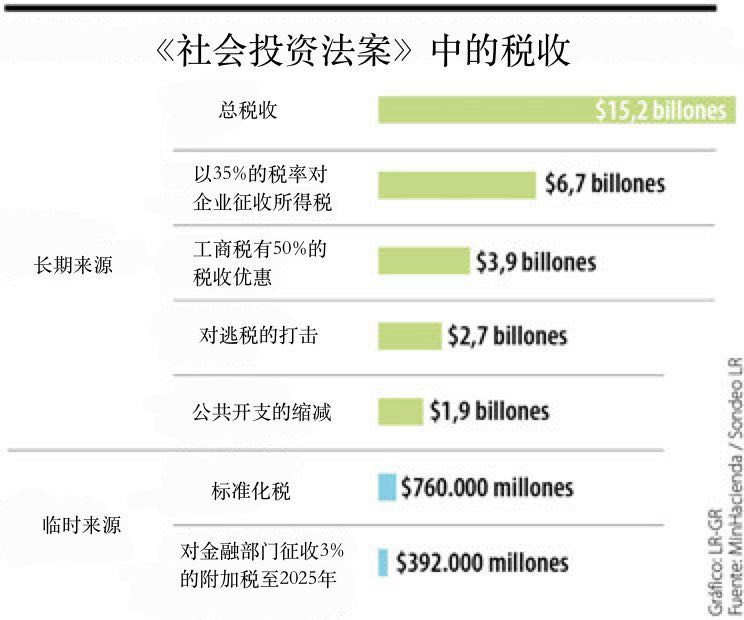
\includegraphics[width=.45\linewidth]{pic/14.jpg}}\\
	\caption{2021年7月税制改革的预计征收目标,图表来源\footnotesize{\url{https://www.larepublica.co/economia/los-asesores-detras-de-los-ponentes-y-coordinadores-del-proyecto-de-inversion-social-3209955}}, 数据来源:哥伦比亚财政与公共信贷部(Minhacienda),制图:LR-GR
}
	\end{figure}
\par 而税收草案二则将征收目标设置为152亿比索,与四月相比下调了约35\%,并且根据财政部计划,这152亿比索的筹集将围绕三个中心:紧缩公共支出、打击逃税漏税和“企业团结”。其中,67亿比索将通过企业所得税征收,而对金融部门征收的3\%的附加税将会额外增加3.92亿的税收;“企业团结”则指将工商税税收优惠由100\%降至50\%,这预计将总共增加39亿比索的税收;而19亿比索将来源于对公共开支的缩减,涉及范围包括官僚开支、人事变动、广告、燃料等方面;另有27亿比索将来源于打击逃税漏税等违法行为,这将通过完善电子发票系统等措施来实现。哥伦比亚财政和公共信贷部部长称,七月的这份提案与其说是“税制改革”,不如说是一项“可持续提供资金的社会支出项目”,是各方面达成的共识,它将“惠及社会最弱势群体,实现财政稳定,为国家经济增长作出贡献” (“Proyecto de Inversión Social busca recaudar \$15,2 billones: Ministro de Hacienda”, 2021)。它将改革的重点从扩大税基转变到“开源”与“节流”并行,而具体措施中则包括许多引人关注的要点,比如节省公共开支和打击逃税等等,而这些分别从不同方面减小了改革的阻力,下文我们将加以具体讨论。
\subsubsection{减少普通民众的负担:对抗议者的让步与妥协}
\par \textbf{(1)税率调整与所得税结构的转变}
\par 税收草案一提出的所得税组成包括个人所得税和法人所得税两部分,而税收草案二则将所得税的纳税重担交给了企业。作出的修改主要有以下几点:第一,法人一般税率从30\%上升至35\%,增加了5\%;第二,四月的法案中,将在2022至2023两个纳税年度对所有企业征收3\%的附加税,但七月的改革提案则缩小了附加税纳税人的范围——只适用于在相应的纳税年度应税收入大于或等于120,000 UVT\footnote[25]{UVT(la unidad de valor tributario),指税收价值单位,2021年设定1 UVT = 36308哥伦比亚比索,数据来源:哥伦比亚国家税务与海关总署文件Resolution No. 000111 of 11 December 2020。}的金融机构,税率为3\%,并且纳税期从原来的2022至2023两个纳税年度延长到2022至2025四个纳税年度\footnote[26]{详见税收草案一:第75、76条;税收草案二:第8条。}。
\par 这一调整带来的直接影响是,最终筹款目标的60\%以上将由企业来完成。其事实依据是,在过去三十年中,哥伦比亚一直是拉丁美洲乃至全世界收入不平等最严重的国家之一,据统计,48.6\%的国民收入由最富有的10\%的人口获得,而最贫困的50\%的人口仅获得国民收入中的12\% (“Wealth and Income Database”, 2021) 而这样的贫富差距受新冠疫情的影响而变得更加严重。在四月的改革中,政府通过扩大税基,使成千上万的哥伦比亚人负担了税款,其中包括收入在中等水平之下的人,而改革方案提出后引发的抗议活动,也恰恰印证了在哥伦比亚这样一个有 350 万极度贫困人口、2100 万贫困人口的国家,通过扩大税基的方式实行税制改革,在社会层面带来的后果是使几乎所有普通民众的生活受到重创,本就微薄的收入再次被削减,随之而来的却是更高的物价和更高的生活和生产成本。人们普遍希望最富有的企业和个人承担起更多的责任。七月的改革方案中的这部分调整正是政府面对抗议活动时做出的妥协。通过这些调整,政府改变了自己的原有目标,满足了一部分抗议者的诉求,以期获得更大的支持和更少的阻力。而这些让步确也从一定程度上减少了抗议。哥伦比亚财政部部长在接受西班牙《国家报》采访时被问及“作为一名官员、新任财政部长和哥伦比亚人,当看到抗议活动时是什么感受”时,而他的回应正体现了抗议者诉求对于契约法案中种种调整的重要促进作用:“非常重要的是,要认识到这种抗议应当得到解决,而解决的方法就是采取一种对话、建立共识和开放倾听的态度……我们整面临着疫情的影响,这次疫情在贫困、失业等关键问题上影响了我们,波及到许多部门。这让人们感到担忧,比如那些年轻人,还有扮演其他社会角色的许多人,这种担忧需要我们来关心和解决。因此,在我们的提案中,我们想要更多地关注社会弱势群体……而受疫情影响,那些小微企业非常脆弱,处于弱势地位。有一点共识是,这个提案不能触碰、不能干涉、不能影响中产阶级。还有一个共识是,我们必须利用商界和最富有的部门所表达的那种团结感,让他们举起手来说:‘我们愿意作出贡献’。”(Cota, 2021) 而对金融机构增加税收则是由于多年来哥伦比亚金融机构的增长一直高于整个经济体系中其他部门的增长。虽然受疫情影响,各金融机构也遭受了损失,但在社会各界的呼声下,他们表示愿意承担纳税义务,为支持哥伦比亚弱势群体所需的社会政策提供资金,助力经济复苏。("Reforma tributaria 2021)
\par 在四月的改革中,政府通过扩大税基,使成千上万的哥伦比亚人负担了税款,其中包括收入在中等水平之下的人,而改革方案提出后引发的抗议活动,也恰恰印证了在哥伦比亚这样一个有350万极度贫困人口、2100万贫困人口的国家,通过扩大税基的方式实行税制改革,在社会层面带来的后果是使几乎所有普通民众的生活受到重创,本就微薄的收入再次被削减,随之而来的却是更高的物价和更高的生活和生产成本。人们普遍希望最富有的企业和个人承担起更多的责任。因此七月的改革方案中的这部分调整满足了一部分抗议者的诉求,能够从一定程度上减少抗议。
\par \textbf{(2)“免增值税日”:适用商品的增加}
\par 在四月的税收草案一中,就已经作出了关于增值税优惠的有关规定——设立“免增值税日”(Días sin IVA)。规定在限定条件下,部分商品每年最多有三天的“免增值税日”。七月的税收草案二仍然保留了这项规定,但是在原有的基础上作出了一些修改,进一步扩大了“免增值税”日所适用的商品范围。
\par 在税收草案一中,适用商品为:服装、服装配件、家用电器、体育用品、玩具和学校用品中销售价格在规定标准以下的部分商品;但是在七月的方案中,适用商品有所增加,规定将“农业部门的物资和商品中每单位销售价格等于或低于80 UVT(不含增值税)的部分”加入“免增值税”日的适用商品范围,并且在后面的说明中指出,这类商品包含种子、肥料、农药、动植物药品、机器等等\footnote[27]{在税收草案一中,适用商品为:服装、服装配件、家用电器、体育用品、玩具和学校用品中销售价格在规定标准以下的部分商品;但是在七月的方案中,适用商品有所增加,规定将 “农业部门的物资和商品中每单位销售价格等于或低于 80 UVT(不含增值税)的部分”加入“免增值税”日的适用商品范围,并且在后面的说明中指出,这类商品包含种子、肥料、农药、动植物药品、机器等等。详见税收草案一:第44至50条;税收草案二:第27至29条。}。
\par 此前,农业方面的税制调整引起了许多争议。四月的税制改革将原本一部分增值税豁免商品调整为增值税排除商品\footnote[28]{增值税豁免商品(bienes exentos de IVA),指需要对其征收增值税的商品,但增值税税率为0,只有该商品的生产者有权抵扣购买或进口该商品所缴纳的税款;增值税排除商品(bienes excluidos),指在商品性质上可能产生增值税、但是根据法律规定并没有被征收增值税的商品,因此产生的“增值税”不能得到抵扣,这部分金额可能进入成本成为其一部分,或成为收入中的可扣除部分。一种商品的种类从前者转变为后者即意味着商品增值税部分的金额被作为成本计入原价,生产者无法在税收上获得优惠。},这些商品包括在人们生活消费中占很大比重的鸡蛋、牛奶、奶酪、鸡肉和猪肉等食品。这意味着许多农业生产者将无权获得生产过程中支付的增值税的退税。哥伦比亚生猪协会会长杰弗瑞·法哈尔多(Jeffrey Fajardo)在接受卡拉科尔电台(Caracol Radio)的采访时指出:“通过将猪肉和其他基本食品,如牛肉、鸡肉、牛奶、鸡蛋和大米从增值税豁免商品转变为增值税排除商品,生产者无法收回生产过程中支付的增值税,因而生产成本提高了,而这最终将通过更高的价格转嫁给消费者,使食品更加昂贵,这与总统在最近几周所确认的‘改革不会涉及哥伦比亚人的食物’相违背。”(“Reforma tributaria 2021: cómo quedará mi bolsillo y qué tengo que saber”, 2021)哥伦比亚政治科学研究院董事会成员安德烈斯·埃斯皮诺萨·芬瓦斯也表示,新的税收负担不仅会导致食品价格上涨,而且会增加农产品的进口,降低了本国农业的竞争力:“哥伦比亚的农业需要税收激励措施来促进农村的就业和重生。”(Fenwarth, 2021)而新的改革方案中,政府在“免增值税日”的相关规定上作出了一些妥协,将农业生产所需的部分商品纳入“免增值税日”适用商品品类,一方面,为占全国劳动力人口17\%的农业生产者带来了一些优惠,能够在一定程度上降低农业生产成本、促进农业发展;另一方面,与之相关的改革最终将传导到农产品物价上,而这则与每一个人的生活息息相关。
\subsubsection{经济复苏与社会福利政策:对抗议者的安抚与拉拢}
\textbf{(1)刺激就业:正式就业支持项目(PAEF)的回归与创造新的就业岗位}
\par 在新冠疫情背景下,哥伦比亚国内失业问题日益突出。有受访者就向我们表示:“疫情使许多行业无法正常运转,所以有许多人正在失业,这就意味着一些家庭失去了收入来源。如果能让那些小公司继续生存下去,这样就能提供更多的就业,有更多的家庭将因此获得更好的生活。”\footnote[29]{参见访谈稿(Julieth):“Muchas familias, por ejemplo, desde que estamos en pandemia o así hay trabajos que ya no se pueden realizar, como se realizaban anteriormente…Al tumbar la Reforma tributaria lo que se hacía era que estas microempresas siguieran sobreviviendo y que estas familias están bien, lo que colocó al proveía mucho más trabajo.”}税收草案二在先前的基础上,将正式就业支持项目延长至2021年12月,并且将重点关注雇员人数小于50人的小企业\footnote[30]{详见税收草案一:第27条;税收草案二:第19条。}。
\par 在四月的方案中,政府鼓励雇主积极增加就业机会,并通过税收减免的方式给予雇主优惠。而在七月的方案中,对于积极增加就业、尤其是年轻人就业的雇主,政府将直接提供奖励,给予其经济上的补贴:“若新聘用的职工年龄在18至28岁之间,雇主将收到国家提供的一笔资金作为奖励,该资金数额相当于每一个新聘职工的每月法定最低工资(SMLMV)的25\%;若新聘用的职工年龄不符合上述限制,并该职工工资在三单位每月法定最低工资(SMLMV)以内,雇主同样将收到国家提供的一笔资金作为奖励,该资金数额相当于每一个新聘职工的每月法定最低工资\footnote[31]{每月法定最低工资(salario mínimo legal mensual vigente, 简称SMLMV)。2021年哥伦比亚的每月法定最低工资为908,526.00比索。}的10\%”,同时,规定该项奖励措持续至2023年8月\footnote[32]{详见税收草案二:第22条。}。
\par 据哥伦比亚财政和公共信贷部部长雷斯特雷波称,这些措施将使得超过731,000名处于极端贫困中的哥伦比亚人受益,预计惠及共330万户家庭。(“Reforma tributaria 2.0 no tocará IVA, pensiones, ni la base gravable”, 2021)实际上,该激励机制后来也得到了落实。2022年2月,哥伦比亚劳动部报告称,在该激励机制影响下,哥伦比亚国内创造了270,142个新的工作岗位。劳动部部长安赫尔·库斯托迪奥·卡贝雷拉(Ángel Custodio Cabrera)发言称:“我们已经见识到了2021年11月和12月实施的就业激励措施。仅在此期间,就创造了79,764个工作岗位,我们将向6,000名雇主支付457.32亿美元,他们将看到政府对此的巨大支持。”(“Incentivo del Gobierno para generación de empleo creó más de 270 mil plazas”, 2021)政府通过增加支出,设置奖励资金,带来的直接影响是企业积极扩充就业岗位,这样的举措有利于减少社会上的失业人口,从而在一定程度上为新冠疫情冲击下低迷的劳动力市场注入新的活力,也间接地帮助一些家庭缓解了经济上面临的难题,一定程度上满足了部分抗议者的诉求,因而有利于减少抗议。
\par \textbf{(2)对高等教育的支持:听见年轻人的诉求}
\par 在哥伦比亚,高质量的教育都不是免费的,且学费相当高昂,因此只有一些相对富裕的家庭能够享受到高质量的教育。对于最好的大学来说,一个学期(三个月)工程学的学费平均在1700万到2000万比索左右(约合人民币30000-35000元),而医学专业可能要2200万到2300万比索(约合人民币38000-40000元左右)。而这仅仅是一个学期的学费,并不包括其他食宿、交通等方面的花销。基本所有大学每年都有两个学期,因此一个大学生一年的学费至少需要4000万比索。而对于很多家庭来说,他们的收入只能达到每年2000万左右。尽管高校也设置了也存在奖学金,但是数量很少,并且因为初高中就出现的教育质量大幅度的分化,穷人的孩子很难因为其综合素质和成绩获得奖学金。在这种状态下,对于哥伦比亚的普通工薪家庭,好的大学是他们所难以触及的。
\par 我们的受访者之一也向我们介绍了哥伦比亚高等教育的具体情况。哥伦比亚的大学分为公立与私立两大类。在公立大学,学生根据自己家庭的实际经济水平支付学费。每年或每两年,政府都会对此做一次普查,会有专员来到学生家里,按照特定评价标准给予该家庭经济水平的评级。公立大学根据家庭的经济水平评级和年收入证明文件收取学费。而私立学校的学费更是远远大于公立大学的学费。她认为在哥伦比亚“大多数人都没有机会接受高等教育”,以及“很多家庭的收入完全无法满足孩子上大学和生活所需”\footnote[33]{详见访谈稿(Julieth)。}。随着越来越多的年轻人加入到抗议中,大学生作为一个群体也提出一些越来越个性化的诉求,其中最为重要的一点便是要求政府免除大学生学费。
\par 税收草案一已对高等教育问题有所涉及:提出“E世代”计划,规定“国家政府每年将拨出资源,为在公立高等教育机构体系中技术学校、职业学校、科技学校和大学中就读的贫困、极端贫困或困难学生支付部分或全部学费”\footnote[34]{详见税收草案一:第29、30条。}。但是此条法令对于“部分或全部学费”的概念界定非常模糊,甚至并未列举附加条款加以具体解释。从后续大量的学生抗议来看,大体可以推知该法令并没有得到很好的落实。
\par 这两条法令在税收草案二中有所调整:“‘零学费’政策和接受高等教育的机会:国家将每年拨出资源,通过支付公立高等教育机构本科生的学费,满足弱势家庭的年轻人的需求。”\footnote[35]{详见税收草案二:第23条。}明确提出了实行“零学费(Matrícula Cero)”政策。对于哥伦比亚大多数收入不高的家庭来说,这无疑大大减轻了他们的经济负担。而在政策的落实方面,我们的访谈对象表示,她和同学们在后来的一个学期完全不必支付任何学费,并且“零学费”政策成为了抗议带来的所有成果中对她影响最大的一项\footnote[36]{参见访谈稿(Julieth):“En cuanto a mí personalmente, (la influencia fue) en la parte de la matrícula 0. No tuve que pagar la matrícula y la verdad es que eso es un descanso para mi mente.”},而这也满足了大多数公立大学学生最主要的诉求。政府在高等教育的学费支付上作出妥协,很大程度上安抚了抗议中非常庞大的公立大学学生群体,有效地减少了学生群体的抗议。
\subsubsection{打击逃税与缩减部分开支:应对财政危机而不激起抗议的其他方法}
\par \textbf{(1)对逃税\footnote[37]{逃税(evasión fiscal),此处为直译,与国内的“逃税”概念可能稍有出入。哥伦比亚国内最常见的逃税形式为以下几种:第一是虚假纳税申报,当纳税人申报收入时,申报的金额较低或不符合实情;第二是将销售额进行拆分,对一部分财产进行转移,从而以较低的税率缴纳增值税,甚至直接设立“空壳公司”来达到逃税的目的;第三是寻找 “逃税天堂(paraíso fiscal)”,即寻找一个税收负担比其他国家低得多的国家,如开曼群岛、摩纳哥、巴哈马等小国,将财富藏匿于此,从而逃过高昂的税收。}的打击:弥补巨额漏洞的一小步}
\par 据统计,哥伦比亚是世界上逃税问题最严重的25个国家之一,每一年的逃税额都数以亿计。据哥伦比亚国家税务与海关总署计算,在2015-2019年期间,逃税金额占纳税总额的比例每年都处于一个相当高的数值,虽然总署声称“逃税率的下降证明了对税收的管理是行之有效的”,但显而易见的是,这样的成效在巨大的数额面前是非常微小的,逃税的总金额仍然居高不下。光是在2019年,哥伦比亚国内的逃税总金额就超过400亿比索,其中,增值税的逃税金额约为207亿比索,法人所得税逃税金额约为216亿比索,而这一年设定的征收总额为1579亿比索。
\begin{figure}[!h]
	\centering
	\vspace{-0.3\baselineskip}
	\subfloat{
		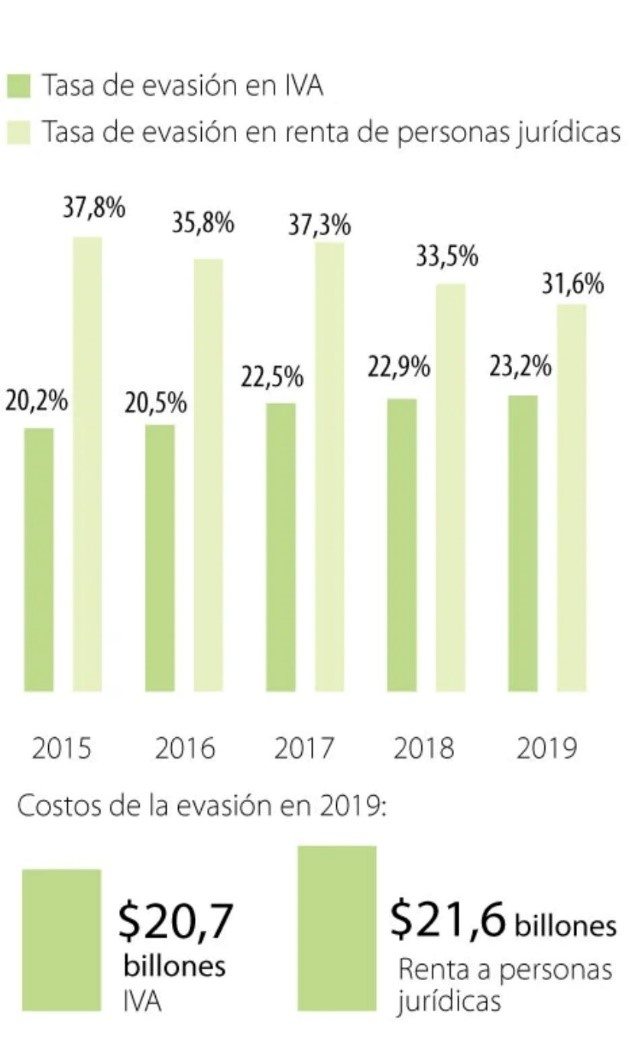
\includegraphics[width=.45\linewidth]{pic/15.jpg}}
	\quad
	\subfloat{
		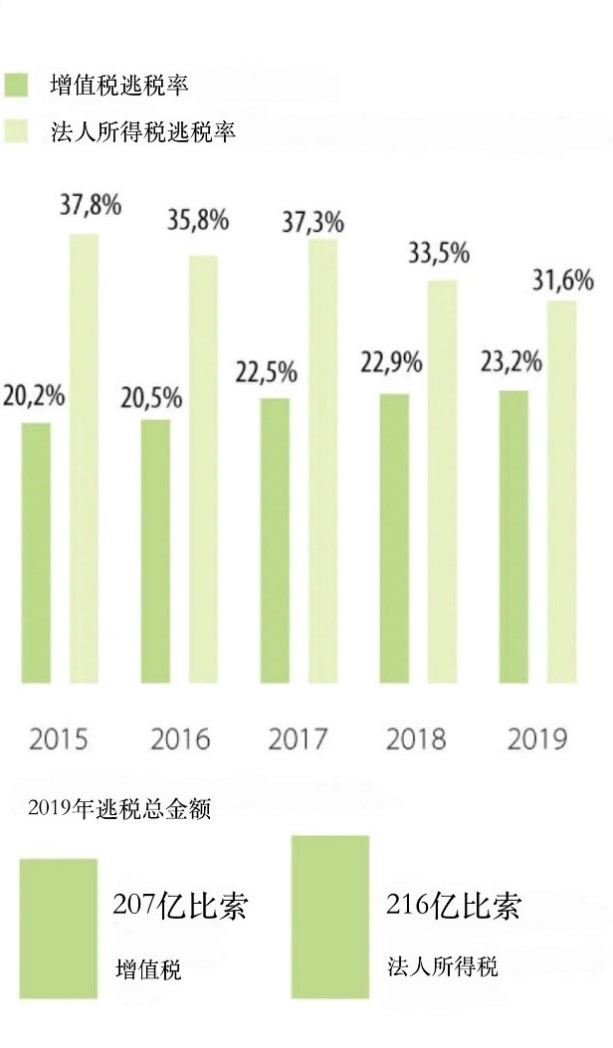
\includegraphics[width=.45\linewidth]{pic/16.jpg}}\\
	\caption{哥伦比亚2015-2019年逃税率与2019年逃税金额,图表来源:\footnotesize{\url{https://www.larepublica.co/economia/evasion-de-iva-e-impuesto-de-renta-es-20-del-recaudo-tributario-en-colombia-3211548}},数据来源:DIAN(哥伦比亚国家税务与海关总署), 制图: LR-VT
}
	\end{figure}
    \par 哥伦比亚国内最常见的逃税形式为以下几种:第一是虚假纳税申报,当纳税人申报收入时,申报的金额较低或不符合实情;第二是将销售额进行拆分,对一部分财产进行转移,从而以较低的税率缴纳增值税,甚至直接设立“空壳公司”来达到逃税的目的;第三是寻找“逃税天堂(paraíso fiscal)”,即寻找一个税收负担比其他国家低得多的国家,如开曼群岛、摩纳哥、巴哈马等小国,将财富藏匿于此,从而逃过高昂的税收。纽约大学阿布扎比分校的哈维尔·梅亚(Javier Mejía)教授认为解决问题的关键在于制度方面,即建立一个相对简单且税率较低的税收系统:“一方面,它通过鼓励按规缴纳税款来降低征税成本;另一方面,它降低了监督成本,使逃税更加困难。”谈起抗议活动,他表示:“最近的抗议活动清楚地表明,企业在不同的政治倡议中并没有受到很好的保护。对政治框架进行巩固,使公司可以在其中开展经营活动而不必担心被征用或受到伤害,这对于鼓励投资也至关重要。这需要该国各方面政治力量作出承诺。”(Cifuentes, 2021)
\par 四月的税收草案一已就此问题对税法的相关条款进行了一系列修改,而七月的草案则将“反逃税”明确为改革的重点之一,并且完善了相关法令。改动内容包括:完善发票系统,在提案第11条中增加规定,发票系统将不再仅仅由销售发票和有同等效力的文件组成,还包括所有由国家税务与海关总署承认的电子文件,并对这部分电子文件作出了一系列补充解释。还规定了电子商务平台应提供条件使平台用户向最终消费者开具电子发票。此外,加强监管房地产销售中的税收,要求公证人严格履行义务,依法确定房地产商业价值。并明确规定,若财产价值严重不符,而公证人并未告知当事人与税务机关,则将按照《税收法规》第651条的规定对其进行处罚。
\par 尽管税收草案二在这方面进行的改动并不是非常大,但通过简化程序、严格监督等措施,足以体现政府打击逃税的决心,这对于不满于税收现状的企业和个人来说,可能起到一定的安慰作用。但是要想根本上解决问题,减少哥伦比亚国内的巨额逃税税款,仍然是社会各界面临的难题。
\par \textbf{(2)缩减开支:自上而下的努力}
\par 改革的另一项重要组成部分是缩减开支与提高效率。这一点在四月有所涉及,到了七月则成为改革的核心之一。
\par 税收草案一中规定,将在国家层面对开支进行缩减。根据法案第33条,自2022年起至2026年,人事开销与国家各机构商品与服务采购费用的年度增长在任何情况下都不得超过中期财政框架中该年的预期通货膨胀目标。而在税收草案二中,紧缩开支的计划年限延长至接下来的十年,并且对此提出了具体方案:第一,逐步减少用于行政活动中用于差旅、文印、宣传、车辆采购以及燃料的费用支出,直到与2019年发生的支出相比达到50\%的减少;第二,不再为任何级别的公务员续订或购买手机和移动电话、互联网和数据服务,并逐步取消目前已购买的服务,并在2023年之前完成这一工作。第三,鉴于远程办公(普及)的情况,考虑逐步减少实体设备租赁的开销,等等。
\par 总体而言,七月的税收草案二将缩减开支这一原本看似是“口号式的号召”加以详细阐述,并将其作为长期工作的重点之一,这是非常引人关注的。哥伦比亚政治家胡安·洛萨诺(Juan Lozano)在四月的税收改革之前评论道:“数以百万计的哥伦比亚家庭作出了巨大的牺牲,他们削减了消费开支,甚至因收入减少而连最基本的生活需求都得不到满足,但我们在国家行政机构中却没有看到同等的努力。当从比较的角度审查公共账户时,与过去十年安相比,国家运营成本显著增加。打击“浪费型国家”的承诺不能淡化。许多私营公司为了生存被迫削减成本、减少工资,这一切痛苦而严重。总之,公共部门也必须做同样的事(削减成本),并且及时交流。”(Lozano, 2021) 在哥伦比亚,人们普遍认为,政府的腐败问题非常严重。根据全球清廉指数的收据,自2011年来,哥伦比亚的得分在36分到39分之间波动(满分100分,100分代表没有腐败,0代表腐败程度很高),2021年在180个国家中位列第87名。 (“Colombia se vuelve a rajar en corrupción según índice de Transparencia Internacional”, 2021)政府增加了税收,但行政效率和福利水平却没有得到明显提高,这让本就敏感的公众的情绪一触即发——税收到底流向了谁的口袋?新冠疫情究竟是财政面临困境的主要原因,还是成为了政府的挡箭牌?我们的其中一位受访者表示,由于政府长期以来的腐败,她对政府的信任度只有一分。“当政府要实行一个项目的时候,中间会有很多人经手,就在这个过程中,钱慢慢地被‘偷走’了;然后等到真的要实行这个项目的时候,已经没钱了,甚至可以说这些项目只是为了掩盖(腐败)而实行的。他们只是说‘对,我们要解决这个地方因为腐败而缺钱的情况’,但事实是腐败持续存在着。”\footnote[38]{参见访谈稿(Julieth):“Hay tantos intermediarios dentro de un proyecto de público que entre ellos se van robando el dinero y cuando ya va a llegar el momento de realizar el proyecto, ya no hay nada, incluso estos programas son como para tapar eso, simplemente dicen “sí existe este programa para poder solucionar la ciudad perdida de dinero debido a la corrupción”, pero la verdad sigue habiendo la corrupción.”}
\par 七月的改革方案预计通过政府缩减开支节省约19亿比索,财政部声称这将是“近几年来政府实行的最重要的节俭措施之一”。这部分措施能够从一定程度上让公众看到一种“自上而下”的努力,也许有助于重建他们对政府的信心。
\subsubsection{改革的总结:有效让步}
从上文对改革总体框架和具体条文改变的分析,可以看到,面对以中产阶级和学生为主的抗议者和反对人士,哥伦比亚政府在多个方面都做出了一定的政策让步和福利项目型的引诱。一方面,政府降低了扩大税基的力度、转而“开源节流”,并更侧重于通过反逃税和减少开支来达成原先税制改革的目的;另一方面,0学费和创造新岗位等政策被正式写入法案,这缓解了青年学生的经济压力,而青年学生正是哥伦比亚抗议的主力军。事实上,第二次政策改革所遭遇的阻力远低于第一次:七月份提出的法案在九月份被正式通过,并于2022年实施。可以说,哥伦比亚政府采取的这类让步引诱型政治控制手段在一定程度上达到了促进政策推行、减少反对阻力的作用。
\subsection{信息操控:污名化宣传与多种审查}
根据Hassan et al. (2022) 对政治控制手段的定义,信息操控是其中的一项重要策略;具体而言,教化是信息操纵的重要组成部分,其定义则并不限于学校内的教育,而进一步包括宣传(propaganda)和审查(censorship)。在哥伦比亚抗议期间,为了减少示威游行,政府所采取的主要宣传类策略是对游行示威者的污名化(stigmatization),在审查方面则综合使用了删除影像资料、断电、阻止影像资料拍摄、威胁影像资料拍摄者等手段。
\subsubsection{对抗议活动污名化的方式与效果}
污名化意指对个人或某一组织的诋毁性行为,旨在通过突出个人或群体身上存在的、或被强制认为存在的某些偏离社会常规的“负面”特征,以达到贬损其价值的目的。污名化的行为常常具有隐蔽性,而难以观测。(Kreiner et al., 2022)在对哥伦比亚游行示威的反应中,我们同样可以看到污名化的存在。其中的一部分是由政府主导、可被观测到的,另一部分则可能更为隐蔽、且难以找到确切的主导者。
\par 可被观察到的、由哥伦比亚政府和政治精英主导的污名化方式主要有三种。首先是宣称并突出有游击队(guerrillas)或其他武装组织参与抗议游行。游击队在哥伦比亚是一项历史遗留问题,其形象在哥伦比亚的群众心中天然带有一定的负面含义: “如果你是游击队员,人们会认为你是一名屠夫、杀手、强奸犯,诸如此类。”\footnote[39]{参见Camilo Mundólogo访谈稿。从人们对曾是游击队员的总统竞选者古斯塔沃·佩特罗的态度中,这种对游击队员的负面印象得到了印证,具体参见Camilo Mundólogo访谈稿: “They might think that Gustavo Petro was once a guerrilla and thus a bad person. ”以及Airi访谈稿: ”Regarding Gustavo Petro, as you asked, many people think he might be the worst candidate out there. Since he has been proven to have some relationship with the guerrillas and that stuff, it's kind of hard to people to believe him and like believe he will make a change for the country.”}因此,通过宣传游击队等武装组织参与抗议游行、或者宣称他们是“幕后黑手”,被视为一种污名化抗议游行的方式。其次,政府会组织警察渗透进抗议组织并挑起暴力和混乱情况,再将此类暴力归咎于游行示威者,以使游行示威进一步蒙上暴力的阴影、以至于让人感觉游行示威者所做的只是产生暴力和混乱 \footnote[40]{参见La Primera Línea Bogotá采访稿: “El tema de los infiltrados de la policía en las manifestaciones es otro de los temas que no se puede ocultar. Había barrios de policías infiltrados, que también llegaban y generaban el caos, generaban la violencia, y pues obviamente hacían que las manifestaciones sean como en un plano de violencia, de que las manifestaciones lo único que generaban era la violencia, por el tema de los infiltrados que pues inicialmente la generaban y pues ya desataban todo el caos y las manifestaciones.” }。尽管此类手段是在非网络宣传领域实施的,但是其根本目的是为了使游行示威呈现出更为暴力和非法的性质、从而使警方镇压显得更为合法,因此也应当被视为一种污名化的手段。另外,将以“前线”为代表的抗议组织统一指称为“恐怖分子”也是一种常见的污名化说法,如哥伦比亚议员玛丽亚·费尔南达·卡瓦尔(María Fernanda Cabal)的儿子胡安·何塞·拉福里(Juan José Lafaurie)在推文上所说:“[‘前线’]是一个威胁国家安全的活跃而危险的恐怖分子组织。”(Lafaurie, 2022)卡瓦尔议员本人也援引视频称,“前线”中的两名“恐怖分子”在2021年6月曾对两人实施强制搜身和“折磨”,因为他们被认定为卧底警察(Cabal, 2022)。
\par 不可否认,哥伦比亚的抗议情形的确为污名化提供了土壤:无论受访者处于何种社会阶级、是否参加了抗议,几乎所有的受访者都提到,有非抗议者利用游行示威制造了混乱、进行抢劫、实行暴力\footnote[41]{参见Airi访谈稿: ” They took advantage of last year protests and liked the violence and the public disorder, it was in my country to rob or like it destroyed and to (paralyze) our public transportation system. There were many armed groups involved, especially in the higher parts of our country. You would see people with like huge weapons that normal people just don't own there, basically, weapons from armed groups. ” 访谈稿(PLB):“En cierto momento, en las manifestaciones había grupos que solo generaban caos, grupos a los que solo les gustaba pues generar violencia, eso no se puede negar,.”};或是有抗议者先对警方及ESMAD或被认为是卧底警察的人发起攻击,采取暴力行为\footnote[42]{参见Julieth访谈稿: “vi en otros casos en las que había personas que también llegan a la plaza y empiezan a provocar a los del ESMAD, entonces empiezan, por ejemplo, a tirarles piedra, a tirarles alguna lata de cerveza y también los agrede.”};或是有游击队支持了部分抗议者的行动\footnote[43]{参见Camilo Mundólogo访谈稿:"I think that there were some infiltrados even with the police and the guerrilla groups. There were some students who were immersed in that revolutionary ideology or something like that. For example, they received some arms or guns from the guerrilla groups and some instructions to do that. I think it’s true."}。但是,突出此类行为的宣传依然应当被视为污名化,因为它试图放大抗议的暴力和非法特征,以期“使人们感到困惑”“操纵人们的想法”“扭曲信息,仿佛人们才是这些损害与糟糕情形的始作俑者”\footnote[44]{详见Camilo Mundólogo访谈稿: “They even tried to find some other ways to manipulate people’s minds and to generate confusion. […] But the people that usually call them terrorists are the people who want to manipulate people’s mind and want to create all this confusion. […] there’re others who twist the information and make people look like the ones who caused all this damage and terrible situation.”}。
\par 另一方面,污名化的效果也较为有限,并非所有接受信息者都会因为这些负面消息而认为抗议的整体特征即是暴力和非法的。游行示威组织是“恐怖分子”的看法并没有受到广泛支持\footnote[45]{详见Camilo Mundólogo访谈稿和Julieth访谈稿。},而受访者也常会指出整体上还是非暴力的示威更多,且几乎所有的示威起初都是非暴力的\footnote[46]{参见Camilo Mundólogo访谈稿:” There were more peaceful protests. As I heard from all the information on social media, violent protests were basically a provocation created by the police or the government. There were more peaceful protests.”}。关于暴力的制造者,也有三种与污名化说法相反的意见:部分社交媒体报道显示,暴力示威主要是渗透的警察引起的;抗议组织者认为,浑水摸鱼者可能并不应当被视为抗议者\footnote[47]{参见La Primera Línea Bogotá采访稿:” pero estos grupos pues no pertenecían a las Primeras Líneas, esto eran grupos pues de persona entrecomillas ajenas a la manifestación, y pues estas personas generaban el caos a veces inicialmente.”}。此外,也有人认为,所谓“游击队参与抗议”的说法是一种谎言\footnote[48]{详见Camilo Mundólogo访谈稿,La Primera Línea Bogotá采访稿和Julieth访谈稿。}。
\subsubsection{综合的审查手段}
审查是政治控制手段中信息控制部分的常见策略。通过各类形式的审查,公民所接受到的不利于政府推行政策、抑制反对意见的信息会有所减少(Hassan et al., 2022)。面对全国范围的抗议游行示威,哥伦比亚政府也采取了综合的审查手段,其中包括制造阻力型审查(censorship through friction)以及制造恐惧型审查(censorship through fear):前者通过删除信息等方式增加人们传播及获得信息的成本,后者则通过威胁信息传播者称他们会受到惩罚,从而增加信息获取与传播的成本,并最终达成审查的目的(Roberts, 2018)。
\par 在传统媒体方面,哥伦比亚政府及政治精英采取的主要审查手段为禁止相关报道。许多媒体的所有人是亲总统的,因此他们会倾向于忽略对政府不利的消息而报道对政府有利的新闻、甚至制造假新闻\footnote[49]{参见William Andres Betancourt Villota访谈稿:” There are some TV news stations that don’t belong to the government but their owners are the friends of the president. They produce fake news or don’t say everything.”}。但有些时候,这样的制造阻力型策略起到了反作用:一些哥伦比亚公民转而在社交媒体上通过观看直播等方式获取信息\footnote[50]{参见Natalia Ibarra Escobar访谈稿:“Recuerdo que la gente empezó a hacer transmisiones en vivo para que todo el mundo conociera los graves disturbios que se estaban presentando ya que en los medios de comunicación común no lo mostraban tanto.”},并倾向于认为社交媒体上的资料才“更真实可靠”\footnote[51]{参见William Andres Betancourt Villota访谈稿:” We have some social medias on which we can see videos, images and understand the situation how the government works and doesn’t work in some parts of Colombia.” 以及Camilo Mundólogo访谈稿:”The thing is that in Colombia you can probably get the most reliable source of information on social media.”}。而相应的,政府也在社交媒体上采取了审查措施,具体体现为删除影像资料。选择性删除(selective deletion)是制造阻力型审查中的常用手段(Zhuravskaya et al., 2020)。哥伦比亚的经验提示我们,这种手段并不仅限于独裁政府:“执政者删除了部分视频和图片,因为他们不想让世界看到真相。他们想限制(这些影像资料)的影响力。”\footnote[52]{参见Camilo Mundólogo访谈稿: “And there were some videos and images on social media deleted by the president and the government because they didn’t want to show the reality to the world. They tried to limit their influence.”}
\par 与此同时,哥伦比亚政府为抑制抗议游行而采取的审查措施也并不仅限于对内容的控制上。为了从源头上遏制信息传播,政府同时采用了制造阻力型和制造恐惧型审查。首先,在波哥大和卡利都发生了游行期间强制断电。这被游行者视为一种制造阻力型的审查手段,因为“显然,(断电之后,)如果有来自警方的袭击或者其他不公行为,人们要想记录并传播这些证据时,会遇到更大的阻力:没有灯光的时候,拍照和录像都会变得更困难”\footnote[53]{参见La Primera Línea Bogotá采访稿: “el gobierno busca en general censura como sea, y pues de ella cortando la electricidad, eso no solo pasó en Cali, aquí en Bogotá también pasó, en varias manifestaciones cortaban la electricidad en las calles, y pues obviamente si había algún ataque del ESMAD o algo así, algún tipo de injusticia, pues será difícil grabarlo, será difícil tener la evidencia, porque pues sin luz es difícil de capturar algún video o foto.”}。此外,警方及ESMAD也会采取向拍摄者喷射气体等一系列措施阻止拍摄影像资料或进行直播的游行者,从而达到阻止信息传播的目的\footnote[54]{参见La Primera Línea Bogotá采访稿:”Si estamos haciéndolo en vivos y esto el mismo ESMAD le tira gases a las personas que estaban grabando, que estaban tomando registro de la manifestación, de alguna otra manera tratando de generar alguna censura.”}。与此同时,ESMAD也会运用制造恐惧型审查:他们会拍摄并登记游行者的面部特征,通过一定的恐吓性行为来增添游行者的心理负担,达成阻止游行者直播和拍摄的目的\footnote[55]{参见William Andres Betancourt Villota访谈稿:” For example, there were policemen who took pictures of your face and tried to identify you.”}。
\subsection{镇压:抗议治安的方式及效果}
镇压(repression)一般指针对反对国家观念、机构和行事方式者而进行的一系列国家行为,内容上包括由政府机构或其附属机构进行的暴力威胁,如骚扰、监视和监管,以及暴力实施,如逮捕、殴打、暗杀、拷问、失踪、强制流放等行为(Davenport, 2007)。镇压的目标则是使反对方失去机动性或彻底消失,其中的诸多措施属于政治控制策略中较为暴力和显著的部分(Hassan et al., 2022)。
\par 在各类型的镇压方式中,以警察为主体的抗议治安(protest policing)得到了最多的关注(Earl, 2011)。具体而说,抗议治安的类型主要分为:警察出现在抗议现场但不采取行动,采取有限措施如沟通协商与交通管制,使用障碍物并进行拦截,肉搏等肢体冲突,使用催泪弹等武器,以及逮捕(Earl et al., 2003)。但是,并非所有的抗议治安都能达到减少抗议游行的数量和激烈程度的目的,在一定情况下会适得其反(Earl \& Soule, 2010; Odabaş \& Reynolds-Stenson, 2018; Castro, 2022)。在哥伦比亚全国性抗议示威期间,可以看到,警察及ESMAD实行了一系列的抗议治安举措,以期起到镇压抗议的效果。然而,在实际经验中,这些举措反而使得抗议中的暴力升级,并成为更多人进一步参与到抗议游行中的理由。我们将讨论这一时期具体出现的抗议治安手段,证明其在一定程度上并没有达到预期的效果、甚至造成了抗议的反噬,并分析其背后的作用机制。
\subsubsection{哥伦比亚抗议治安手段概述及效果假设}
自2021年4月28日起,抗议游行在哥伦比亚全国各地都频繁发生;相应的,哥伦比亚警方及ESMAD采取的抗议治安措施也非常多样,且在各地抗议中相当普遍\footnote[56]{参见Airi访谈稿:” So there are actually a lot of cases of police violence reported during the protest last year.” 在访谈稿原文中,受访者采用了警察暴力(police violence)的说法。应当指出,并不是所有的抗议治安措施都是警察暴力行为。我们将在后文论述怎样的措施会被识别为警察暴力。不过,我们认为,警察暴力事件的普遍及频繁发生可以在一定程度上反映抗议治安措施的普遍及频繁发生。}。此外,其暴力特征也非常突出,“警方对抗议游行的参与者做了挺过分的事情,尤其是对那些处于最前线的人” \footnote[57]{参见Airi访谈稿:” But the police did really harsh things to people in the protest, especially those in the frontline.”}“他们使用了暴力以恐吓街上参与游行的群众”\footnote[58]{参见William Andres Betancourt Villota访谈稿:” The police used violence to intimidate people in the streets and in the mobilizations.”}。部分游行者被逮捕并被拘留一天至一周\footnote[59]{参见William Andres Betancourt Villota访谈稿:” And then they’re caught by the police and sent to jail for one night or one week.”};ESMAD多次使用了催泪弹和被称为“毒液”(venom)的气体武器,对参加游行者与旁观人士进行了无差别攻击\footnote[60]{详见La Primera Línea Bogotá采访稿及Julieth访谈稿。};有游行者的头部被抛射物攻击而眼部受重伤,此外也有人因ESMAD不规范使用武器而死亡\footnote[61]{详见William Andres Betancourt Villota访谈稿:” I have a friend who lost one eye because she got a stone or metal piece against her head. In other places like the capital or other states bigger than mine, things are more complicated because there’re people or students killed.”以及Jose访谈稿:” But there was a situation in which a policeman shoot a guy here in the back, and he died because of that. But that wasn't supposed to happen.[…] They found out that this type of guns, I mean they can use them in China, in USA, in everywhere. But the problem is that they are not supposed to shoot to the head, they are supposed to shoot to the body.”}。自2021年4月28日起,在卡利等地,抗议治安措施导致游行者死亡的案例并不罕见\footnote[62]{详见William Andres Betancourt Villota访谈稿、Airi访谈稿、La Primera Línea Bogotá采访稿及Julieth访谈稿。};此外,据称部分游行者被带走,被强制失踪并遭到暗杀\footnote[63]{详见William Andres Betancourt Villota访谈稿及La Primera Línea Bogotá采访稿。}。
\par 那么,这一系列抗议治安手段在减少抗议、减少政府推行政策的阻力方面成效如何?Ives和Lewis(2020)指出,在近期发生过镇压后,新的抗议游行中更容易出现暴力升级的现象。我们需要谨慎处理此处的“镇压”概念:应当指出,在2021年4月28日至今的哥伦比亚游行示威中,警方与游行者的对抗显得无可奈何:“有时游行者会影响公共交通的运行等,而警察所受到的指令就是不顾一切代价阻止这些人。最终,双方一定会有对抗发生。”\footnote[64]{详见Camilo Mundólogo访谈稿。} 但是,双方的对抗并不等同于此处的“镇压”,也不必然意味着游行会变得更暴力。那么,怎样的镇压措施会产生如此反效果呢?根据Earl和Soule(2010)的研究,并非所有的抗议治安行为都会对减少抗议数量及其暴力程度产生反作用。事实上,只有同时大量进行逮捕和暴力攻击的抗议治安措施才会引发抗议的进一步“反噬”。
\par 通过前文对哥伦比亚政府采取的抗议治安措施分析可以发现,由警方实施的暴力行为占据了较为显著的部分。因此,我们不妨作出假设:在减少抗议游行的数量和激烈程度方面,哥伦比亚政府采取的这些带有警察暴力色彩的、针对抗议活动的镇压所能起到的实际效果相当有限,甚至可能有反作用。这一假设已经获得了一定的经验支持:实际上,通过访谈可以得知,呼吁人权、反对警察暴力确实成为了后期抗议的主题\footnote[65]{参见La Primera Línea Bogotá采访稿:“durante las manifestaciones entonces pues empiezan el tema de los desaparecidos y asesinatos, violaciones por manos de la policía y el ESMAD, entonces estos se convierten en nuevas razones para salir y pues manifestarse.” 以及Julieth访谈稿:” se pedía mucho respeto hacia los derechos humanos porque es lógico que estén solicitando que respeten sus derechos humanos de los descendientes y sí mismo.”}。下面,我们将运用量化方法,进一步说明这一现象及其背后机制。
\subsubsection{适得其反的镇压:来自数据的证据}
为了检验前文提出的假设,我们收集了来自哥伦比亚25个大区 (Departamento) 首府和首都区 (Distrito Capital) 的暴力抗议及警察暴力数据来进行验证,未被纳入分析的单位在此次事件中没有发生暴力抗议或警察暴力。在数据的选取方面,我们认为,警察暴力作为一种极端的抗议治安措施,可以在相当程度上代表前文结论中所说的“同时大量进行逮捕和暴力攻击的抗议治安措施”\footnote[66]{关于警察暴力与一般抗议治安措施的区别,我们将在后文进行讨论。}。
\par \textbf{(1)测量暴力抗议}
\par 对于暴力抗议,我们使用了ACLED中标记为“Violent Riots”的抗议,数据的时间范围为4月28日至8月2日;并按次国家层面单位进行整合,这样做可以将其他按次国家层面单位核算的变量纳入模型。
\par 观察数据后我们发现,暴力抗议呈现高度右偏的分布,并且伴随着一些0和负值。为了满足小样本OLS回归对误差项正态性的要求,我们使用了逆双曲正弦变换 (Inverse Hyperbolic Sine Transformation, 下文简称IHS)使得变量的分布更近似正态分布,且该变换对0和负值不敏感。
\par \textbf{(2)测量警察暴力}
\par 对于警察暴力,我们使用了GRITA (Grabar, Registrar, Investigar, Triangular, Asistir)出版的关于的哥伦比亚警察暴力的年度报告 (GRITA, 2022),并按上文所述方法进行整合。GRITA为哥伦比亚一家专门收集警察暴力信息的非政府组织,信息源为受害者或者目击者的举报,相比ACLED(主要收集新闻媒体的报道)和政府官方数据有更高的可信度。同样地,警察暴力的数据也高度右偏的分布,并且伴随着一些0和负值,所以我们也进行了IHS变换。变换后的系数解释为弹性,具体的公式则依据Bellemare和Wichman (2020)提出的方法。
\par \textbf{(3)协变量}
\par 我们在模型里也加入了其他可能影响暴力抗议数以及警察暴力数的协变量。首先,我们加入了城市在新冠疫情中的经济衰退情况(2021年各个城市的GDP相对2019年的下降情况),数据来自哥伦比亚国家统计局 (Departamento Administrativo Nacional de Estadísticas, 2022),这样便考虑了疫情带来的短期冲击。其次,我们纳入了各个城市在2019年和2020年抗议\footnote[67]{发生于2019年11月21日至2020年2月21日。}中的抗议数(包含了ACLED中所有类型的抗议)作为滞后变量,因为过去两年的抗议数与2021年的暴力抗议和警察暴力数都高度相关,说明这其中可能包含一些我们没有观测到的信息。最后,我们加入了城市的人均GDP的对数值和人口的对数值,数据来自哥伦比亚国家统计局和世界人口评论 (World Population Review, 2022);过去的研究告诉我们,因为使用暴力的机会成本更低,暴力更有可能发生在贫穷的地区 (Collier \& Hoeffler 1998, 2004)。
\par \textbf{(4)结果}
\par 回归的结果在一定程度上验证了之前的假设,警察暴力对暴力抗议有着显著的正向影响。我们采用了逐步放置变量的方法,在每个模型里人均GDP和人口都有着一定的解释力。模型一只纳入了警察暴力;模型二里警察暴力在其他模型逐步加入控制变量后仍然保持统计显著并有着理论意义;模型三放入经济衰退后系数没有发生变化,而警察暴力的标准误增加,说明经济衰退对结果毫无解释力也没有起到控制其他协变量的作用,这表明疫情的短期冲击对于暴力抗议和警察暴力的关系没有明显的影响;模型四纳入19-20年抗议数后,警察暴力的系数有了一定变化,说明过去的抗议数控制了一些地区性的混杂因素。
\par 为了使得结果更加稳健,我们还进行了残差正态性检验和异方差检验\footnote[68]{将估计值转换为弹性使用了Bellemare and Wichman (2020)提出的方法。对于因变量、自变量都做了IHS变换的情况,弹性$\epsilon\approx\beta\cdot\dfrac{\sqrt{y^{2}+1}}{y}\cdot\dfrac{x}{\sqrt{x^{2}+1}}$。标准误的计算使用$\delta$方法。},其中残差检验显示数据在调整后仍然存在小幅度的右偏,这不会严重影响我们的结果。最后,我们仍然无法排除反向因果的可能,这将在后文进行讨论。
\begin{figure}[!h]
                    	\centering
                    	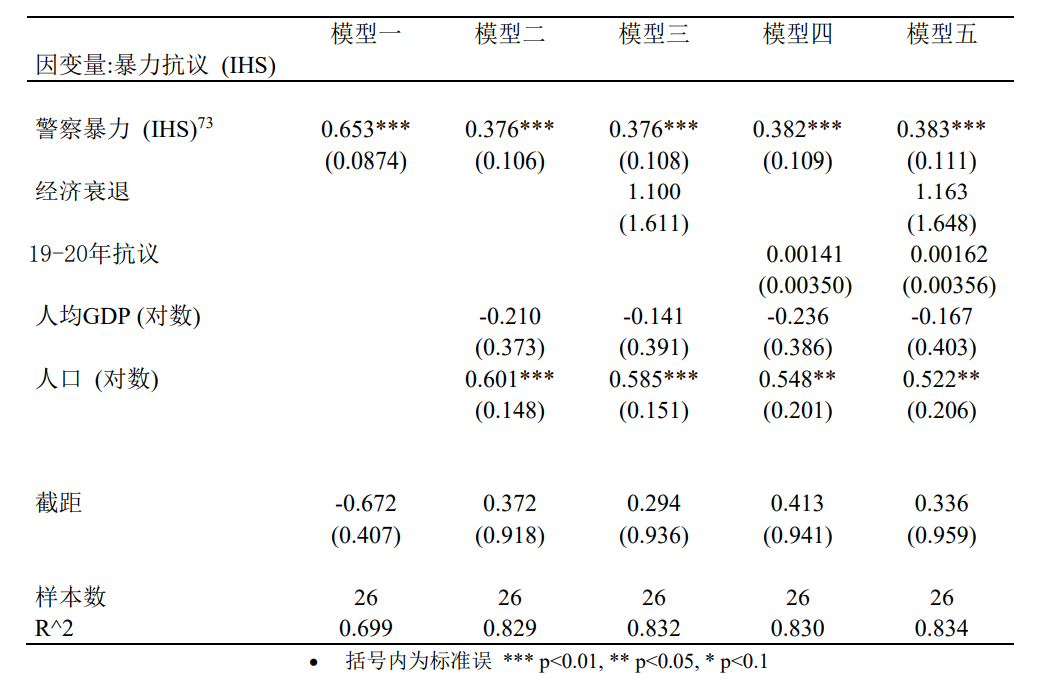
\includegraphics[width=.9\linewidth]{pic/17.png}
                    	\end{figure}
\subsubsection{抗议暴力升级的背后机制分析}
证明了哥伦比亚政府采取的暴力抗议治安措施对减少抗议并降低其激烈程度的反作用之后,我们想要探究的是,为何暴力镇压反而可能导致抗议暴力升级?Castro(2022)为我们提供了理解这种镇压之反作用的三种维度:以抗议治安为代表,镇压的可见性(visibility)越高、武断性或无差别攻击性(arbitrariness)越强、正当性越低(legitimacy),就越容易产生反效果(backlash),从而使抗议进一步升级。首先,镇压行为的影像资料在社交媒体上的传播会增加镇压措施的可见性;此外,以哥伦比亚警方及ESMAD使用催泪弹和“毒液”等气体武器的做法为例,类似的抗议治安手段被视为具有较强的武断性,因为无论是没有使用暴力的游行者还是路过的旁观人士都可能遭受其攻击。因此,这些措施都有可能使哥伦比亚警方采取的抗议控制措施失效或起到反作用,进一步催生游行的暴力升级、让更多的人参与抗议。另外,对于抗议治安的正当性判断也是镇压能否达到预期效果的重要影响因素。
\par\textbf{(1)可见性与社交媒体}
\par 社交媒体对2021年4月28日起哥伦比亚全国抗议游行的组织者和参与者的重要性不言而喻。首先,社交媒体为举行抗议游行活动提供了极大的便利:多数抗议者都通过Whatsapp, Facebook和Instagram等社交媒体获得并传播抗议活动的时间、地点等信息,达成聚集并集体参与游行的目的\footnote[69]{详见William Andres Betancourt Villota访谈稿:” We keep in touch on social media. There were some groups of student leaders who organized the mobilizations and the strikes. They sent the information and details of the protest, like when to go and where to go, on social media.”La Primera Línea Bogotá采访稿:” Through whatsapp, it is the main social media I use. It is like, a friend sends you a message and tells you that there is a protest tomorrow, where we are going to meet and then start. Another social media is Facebook.”以及Julieth访谈稿:” cada quien cada grupo convoca estas manifestaciones en sus puntos, en sus zonas, normalmente por las redes, tanto Facebook como Instagram, zonas de redes en las cuales pues más se mueve la información. También hay grupos en Whatsapp o en telegram, hay grupos en los cuales también se difunde esta información. Es como la única forma de difusión o de transmitir la información sobre las protestas o cualquier tipo de información. Pues se hace normalmente por las redes.”}。然而,社交媒体对抗议活动的“帮助”并不仅限于此。抗议的组织者强调,对抗议活动进行直播并传播涉及抗议治安中暴力措施的影响资料,是非常重要的:“当警方和ESMAD有不公正的行为时,要传播视频等信息,以让被捕的人不会轻易受到惩罚,并让更多的人看到究竟发生了什么[...]无论这些不公正是在哪个城市发生。[...]要在推特(Twitter)打上标签(tag),将它们分类。[...]这对我们来说帮助很大。”\footnote[70]{参见La Primera Línea Bogotá采访稿:” Muchas de las veces es difundir también la información, muchas de las veces que hay represión por parte de la policía y el ESMAD, la idea es cuando hay pues estos videos y estas fotos es difundirlo al máximo para que la gente los vea, para que se vuelva virales, y pues no quieren como la impunidad. entonces tratamos de difundir la información al máximo para que muchos casos no que impune y pues la gente se entere de lo que está pasando. Independientemente si el caso fue en Cali, en Medellín, en Pereida, la idea es que vamos a difundir la información sin importar la ciudad, entonces pues digamos que normalmente nos compartimos ese tipo de información, o nos etiquetamos, ponemos los tags, para etiquetarlos y pues que puedan compartir la información, pues eso es de gran ayuda.”}
\par 为什么这些通过社交媒体实现的信息传播对遭受镇压的抗议组织者而言“帮助很大”?Odabaş和Reynolds-Stenson(2018)指出,通过社交媒体实现的镇压中“不公正”现象的传播可以让更多的旁观者或不知情人加入到抗议游行的行列中来;由此,社交媒体实际上使得针对抗议的镇压行为更难以达到预期的效果,甚至更容易产生反作用、激发抗议升级。换言之,社交媒体使得抗议治安行为获得了更高的可见性:更多人可以在更大的范围上更直观地看见抗议及其被镇压的情况。而可见性的增加使得抗议治安等镇压行为更容易产生“镇压越强,抗议越多、越暴力、规模越大”的反效果。
\par \textbf{(2)武断性:气体武器,“可他们什么都没做”}
\par 在哥伦比亚政府的抗议治安手段中,有许多呈现出较强的武断性,并且被抗议者及抗议的旁观者所感知。除去前文提到的催泪弹以及无差别攻击武器“毒液”之外,武断性的另一个方面体现于,虽然有“浑水摸鱼”、在抗议中制造混乱和暴力的人,但更多的游行者“什么都没做”。尽管如此,没有任何暴力行为的抗议者甚至旁观者没有在暴力对抗中得到应得的庇护,甚至遭到了攻击。“我什么都没做,没有砸玻璃,没有武器,但我很害怕,我从来没遇见过催泪弹,因此我向一位属于ESMAD的先生寻求帮助。[…]但他所做的是对我采取防暴措施,并打我,而我怕得要死”\footnote[71]{参见Julieth访谈稿:“Y yo quería explicarle a uno de ellos que yo no estaba haciendo nada, que yo no iba a romper un vidrio, que yo no iba a prender juego, que no tenía nada, que si quería que me podía requisar, que yo no tenía nada, que por favor como que me ayudara porque me daba miedo, nunca había estado cerca de los laques, de los gases, lacrimógenos en mi vida. salí corriendo a pedir ayuda a un señor del ESMAD, y lo primero que hizo fue ponerme la protección y golpearme, entonces ahí me di cuenta que no puedo confiar en ellos, yo estaba muerta de miedo, porque había gases lacrimógenos corría hacia el ESMAD, aquí (pide que) me ayudara y lo que hicieron ellos fue golpearme.”}“在很多和平游行中,警方使用了诸多武器,但是没有任何组织保护那些参与了抗议(却手无寸铁)的哥伦比亚人”\footnote[72]{参见William Andres Betancourt Villota访谈稿:“For example, in many Pacific Mobilizations and protests, they(the police) used the tanks and other arms, but there’re not organizations protecting the Colombians who joined the protest.”}“一位老先生,是位大学教授,有着非常美好的生活,[…]但他仅仅因为参加了抗议就被杀害了”\footnote[73]{详见Airi访谈稿。此外,Julieth访谈稿中的受访人Julieth提到一个案例:一位ESMAD的队员在对为保护个人信息而蒙着脸的抗议者实施驱逐和暴力行为时,发现其中的一位抗议者是自己的儿子,于是马上转而帮助他。这也从侧面反映了ESMAD与警方的镇压抗议行为具有相当的武断性。}。
\par 这种显著的武断性可能是哥伦比亚政府抗议治安手段起到反作用的重要原因。警方“毫无理由”的暴力行为激起了他们的愤慨情绪,因而使得诸多和平抗议发生了暴力升级,“很多人不支持(警方投射催泪弹等暴力行为)这些,这让他们非常愤怒、愤慨,所以出现了土炸弹、互殴、破坏商店和城市的行为等等。我认为,很多时候青年人想要的是和平的抗议,但是ESMAD毫无理由地攻击了他们,这让他们感到很愤怒”\footnote[74]{参见Julieth访谈稿。},因此发生了暴力升级。
\par \textbf{(3)抗议治安措施的正当性判断以及愤慨情绪}
\par 并非所有使用武力的抗议治安措施都是警察暴力(violencia policial),而正当性的维度可以帮助我们理解警方合法合理(legal or legitimate)使用武力(fuerza)与警察暴力的区别(Lerchundi, 2020),从而揭示为何含有警察暴力特征的抗议治安措施对哥伦比亚抗议镇压的作用适得其反。根据Jobard(2018)对警察暴力的定义,“过度使用武力”、采取与想要达成的目标或实行警察干预的动机严重不匹配或不成比例的武力措施时,以及在没有危险或未受威胁的情况下使用武力时,其武力行为应被认定为缺乏正当性,属于警察暴力。
\par 针对正当性的前一项判断,人们普遍认为,无论是否有意,造成抗议者死亡的镇压手段是不可接受的\footnote[75]{参见Jose访谈稿。在所有受访者中,该访谈的受访者Jose对抗议者持有的批判态度最为明显,并且对警察使用武力表现出了支持。然而,Jose也认为,造成抗议者死亡“是一个问题”。}。然而,要判断警方是否是在没有危险或未受威胁的情况下使用武力,就不得不涉及到一个重要又难以回答的问题:谁先动的手?从抗议的参与者到旁观者,人们往往会根据自己的倾向做出不同的判断\footnote[76]{其中,Camilo Mundólogo访谈稿与Jose访谈稿的差别尤为明显。}。这一方面说明了正当性判断的重要地位,另一方面也说明,当镇压行为的正当性不够清晰、而显得模糊且难以被判断时,该行为——无论其合法性“实际上”是高还是低——依旧会适得其反:在实际情况中,这种无法确认起始方的暴力行为引起了双方间无休止的“以眼还眼”,使得游行的暴力程度进一步升级:“如果警方进行了暴力攻击,游行者就会回以暴力”\footnote[77]{参见William Andres Betancourt Villota访谈稿。}“这些人能对警方投掷炸弹吗?[...]如果有人对你施以暴力,你得做出回应,不是吗?[...]如果有人突然在街区进行暴力行为,警察得保护其他人、维持秩序”\footnote[78]{参见Jose访谈稿。}。
\par \textbf{(4)对信息操纵的再审视:确保镇压效果的工具}
\par 既然针对抗议所进行的镇压行为之可见性、正当性、武断性会影响其对减少抗议数量及激烈程度的作用,那么相应的,政府也应当可以通过降低可见性、提升正当性、降低武断性的方式来使抗议治安行为更为有效,并避免反作用。需要注意,作为哥伦比亚政府同时采用的政治控制手段之一,镇压与其他策略并非没有联系。不妨重新审视哥伦比亚政府实行信息操纵的原因:为从源头或在途径中阻止暴力镇压相关信息的传播而进行的审查,是一种降低暴力镇压之可见性的手段;同时,将部分非抗议者的暴力行为归咎到抗议游行者身上,突出抗议者暴力特征,从而让抗议活动整体呈现出暴力与混乱色彩的污名化手段,可以增加各类抗议治安行为的正当性、并降低其武断性:“这是政府的一种策略,它让学生[游行者]看上去像是破坏一切的恶人,而警察是哥伦比亚的超级英雄”\footnote[79]{参见William Andres Betancourt Villota访谈稿:“This was like a strategy that the government said the students were bad people who destroyed everything while the police were the superheros of Colombia.”}。
\subsection{讨论:抗议及其反制的其他问题}
\subsubsection{疫情冲击}
如前所述,新冠疫情带来的经济衰退对于暴力抗议\&警察暴力的关系没有显著的影响,这排除了短期疫情冲击的作用作为另一种机制的可能,使得我们的结果更加稳健。
\subsubsection{遗漏变量}
因为数据匮乏,我们的OLS回归模型里未纳入抗议是否有组织(Ives \& Lewis, 2020)、政府腐败 (Neudorfer and Theuerkauf , 2014)等信息,而这可能和暴力抗议、警察暴力高度相关,因而会对我们的结果造成一定的威胁。
\subsubsection{反向因果}
仅仅依靠数据我们无法给出暴力抗议和警察暴力之间确定的因果关系,因为暴力抗议也往往会导致政府使用更加强硬的镇压措施。如前文所述,双方间无休止的“以眼还眼”的暴力行为本就无法确认起始方。但是结合以往的研究和访谈,我们仍然可以相信警察暴力至少在一定程度上导致了抗议暴力升级。
\subsubsection{为什么会有警察暴力?}
作为对上一个问题的补充,我们在此讨论警察暴力行为的可能原因。
\par \textbf{(1)警察暴力的自发性}
\par 这一点也在访谈中得到了印证:警察大多来自中下阶层家庭,从小在充满暴力的贫民窟中长大,这无疑会影响他们之后的行为,特别是在本身就倾向于使用暴力的警察工作中\footnote[80]{参见AIRI访谈稿: “But most policemen are from lower classes, because those are the only jobs they can like afford to apply for. So, they grow up in this violence environment, in this harsh environment, without resources, without public services, where they had a lot of violence going like against them. So, they obviously had an influence since their childhood of a violence environment that may also like be reflected on their actions their behavior when like in their job, in their work.”。关于警察的贫穷和腐败,可参见Jose 访谈稿:“But we can say the people they are in the police are poor people. They are always looking to, I mean their salary is not enough for them, so there gonna be all ways of corruption.”}。
\par \textbf{(2)街头官僚理论}
\par 警察暴力的自发性告诉我们有些警察只是单纯喜欢施暴,然而访谈告诉我们,另一部分人是为了完成工作不得不这么做,只是为了展示自己在做事、在完成本职工作、在镇压,这是政府的要求\footnote[81]{参见La primera linea采访稿:“Bueno, pues normalmente como algunas veces lo hemos dicho nosotros mismo, cuando estamos en medio de los enfrentamientos, (los que) nosotros normalmente salimos y realizamos en vivos en los cuales interactuamos con las personas que escriben y preguntan o opinan, pues normalmente la policía está en la mano con el gobierno, entonces igual como te hablo con el tema de los falsos positivos, o sea, si el gobierno pide resultados, pues muchas de las veces en contra de la voluntad de algunos policías: no todos, porque muchos disfrutan de hacer daños, a muchos se les ve en la cara la felicidad de disparar un arma. Pero hay algunos que se ven como en contra de su voluntad y que tienen que igualmente salir y reprimir al pueblo para de alguna manera mostrar resultados de que sí están haciendo algo. ”}。过去的研究同样证实了这点:警察的暴力行为有时是“做给”同僚、尤其是上司看的,以证明自己在完成某些正式或非正式的“规范动作”,通过此种方式,他们可以获得补贴、奖金或者假期(Lerchundi, 2020)。而一位访谈者指出,警察总是虐待青年人(maltratando)。这似乎是一位警察与青年们相处的常规方式(forma regular),假如ta不暴力对待青年的话——这是警察-青年关系的标准模式——ta可能被看作没有完成本机构的工作规则。以上的发现也呼应了被广泛用以解释基层公职人员行为的“街头官僚”(Street-level Bureaucracy) 理论(Lipsky, 1980),并提供了其在暴力文化盛行的国度的具体解释。
\section{结论}
自2021年哥伦比亚反税制改革示威运动爆发以来,哥伦比亚政府采取了综合的政治控制手段来平息这场全国范围内大规模的社会动乱。一年以来,本小组一直在关注这一示威活动的发展,社交媒体上的相关舆论以及政府采取的相应措施。本小组利用语言优势,发挥不同专业背景的相关优势,通过跨学科的研究方法探究抗议和政府措施的互动,特别是政府政治控制手段对抗议示威活动的影响。
\par 2021年示威运动的导火索是4月28日通过的新税制改革法案,这一改革仅仅在几天后,在巨大的民意压力下即宣告停止, 因为该改革试图在经济不景气的情况下扩大税基、增加面向哥伦比亚普通群众的税收,对以中产阶级为代表的一大批哥伦比亚公民的生活产生了较大的负面影响。而在九月,政府再次通过了另一个税制改革法案,却几乎没有引起人们的反对。本小组同学通过细致的文本分析,对比两份税制改革法律文本的内容,指出政府所做出的妥协与让步: 政府删去了诸多争议性条款,通过开源节流而非扩大税基的方式达成偿还国家债务的目的,并增添了针对学生和年轻劳动者的法定福利项目,以期达到拉拢或引诱公民、降低反对力量的目的,且颇具成效。这些措施在平息抗议游行方面显然获得了很好的效果。
\par 另一方面,妥协与让步并非哥伦比亚政府采取的唯一政治控制方式。通过访谈,本小组成员注意到,为平息抗议活动,哥伦比亚政府也采取了非常多样的信息控制措施:放大抗议者及非抗议者的暴力行为、宣称有游击队参与,以期对抗议实行某种程度的污名化,并通过断电、删除影响资料等方式限制不利于警方对抗议进行治安管理的信息在社交媒体等公共领域的传播。与此同时,警察及 ESMAD也对抗议游行活动进行了直接镇压,而在警方使用的抗议治安手段中,可以看到明显的暴力因素:逮捕并殴打游行者、使用催泪弹等气体武器,社交媒体上不乏游行者在镇压中死亡或被强制失踪及暗杀的案例。然而,这一系列政治控制手段、尤其是由警察及 ESMAD 进行的抗议治安策略,其成效仍有待商榷。
\par 基于此,本小组通过量化的方法,收集了来自政府、权威机构和非营利组织的多方数据,对警察暴力和示威运动之间的关系进行了考察。我们发现在2021年哥伦比亚的示威抗议中,警察采取的治安暴力对平息抗议游行的效果非常有限,甚至起到了激起更多抗议的反作用,并推动了冲突暴力程度的升级。结合访谈中的信息和叙述,可以看到,在抗议者普遍使用社交媒体的情况下,哥伦比亚警方采取的治安手段具有较高的可见性、较高的武断性和较低的正当性,而这会使得镇压的效果适得其反。事实上,抗议的目标的确从一开始的反对税制改革,逐渐转向对杜克政府的批评,并以对警察暴力的批判作为核心。
\par 在 2021 年 4 月底到 5 月初的大规模游行后,抗议示威的声音虽然有所衰减,但也从未离去。同样持续存在的,还有批评抗议示威者的声音。需要指出,本小组的研究面临访谈样本较少和访谈对象立场多样性较为缺乏的问题,同时在获取警察暴力的面板数据时受到了一些阻力。与此同时,本小组的研究着眼于探索哥伦比亚政府为平息抗议活动而采取的政治控制手段及其实际效果,但在分析哥伦比亚政府为何采用特定的政治控制手段,尤其是为何采用暴力的抗议治安手段方面讨论较少。此外,警察暴力何种程度上是机构行为、又从何种程度上是个人行为,这种个人行为又如何扎根于哥伦比亚的政治结构和社会现实之中,值得进一步研究。
\par 无论如何,哥伦比亚的暴力文化传统和贫富差距依然是困扰哥伦比亚公民的重要问题。有些人期待着今年的总统大选,期望哥伦比亚能迎来一位可以“为国家带来改变的” 新总统,我们也如几十年前的伯恩斯一样坚信:“积极的变革应该而且必将发生”(Burns, E. Bradford,1989)。
\clearpage
\addcontentsline{toc}{section}{参考文献}
\begin{thebibliography}{100}
\bibitem{}
{Hassan, M., Mattingly, D., \& Nugent, E. R. (2022). Political control. Annual Review of Political Science, 25(1),\url{https://doi.org/10.1146/annurev-polisci-051120-013321}}
\bibitem{}{Ives, B., \& Lewis, J. S. (2020). From rallies to riots: Why some protests become violent. The Journal of Conflict Resolution, 64(5), 958-986. \url{https://doi.org/10.1177/0022002719887491}}
\bibitem{}{Odabaş, M., \& Reynolds-Stenson, H. (2018). Tweeting from gezi park: Social media and repression backfire. Social Currents, 5(4), 386-406.\url{https://doi.org/10.1177/2329496517734569}}
\bibitem{}{Earl, J. \& Soule, S.A. (2010). The Impacts of Repression: The Effect of Police Presence and Action on Subsequent Protest Rates. (Ed.) Research in Social Movements, Conflicts and Change (Research in Social Movements, Conflicts and Change), 30, 75-113.\url{https://doi.org/10.1108/S0163-786X(2010)0000030006}}
\bibitem{}{Kreiner, G., Mihelcic, C. A., \& Mikolon, S. (2022). Stigmatized work and stigmatized workers. Annual Review of Organizational Psychology and Organizational Behavior, 9(1), 95-120.\url{https://doi.org/10.1146/annurev-orgpsych-012420-091423}}
\bibitem{}{Juan José Lafaurie [@LafaurieCabal]. (2022, April 4). Neutralizar a la Primera Línea debe ser una prioridad para el Estado colombiano: son un grupo terrorista activo y peligroso [Tweet]. Twitter. \url{https://twitter.com/lafauriecabal/status/1510824751824085004?s=21}}
\bibitem{}{María Fernanda Cabal [@LafaurieCabal]. (2022, April 4). Los terroristas de la “primera línea” alias “Calarcá” y alias “19”, coordinaron la tortura de dos personas el 4 de junio [Tweet]. Twitter.\url{https://twitter.com/mariafdacabal/status/1510803413411500037?s=21}}
\bibitem{}{Roberts, M. E. (2018). Censored: Distraction and diversion inside china's great firewall. Princeton University Press.}
\bibitem{}{Zhuravskaya, E., Petrova, M., \& Enikolopov, R. (2020). Political effects of the internet and social media. Annual Review of Economics, 12(1), 415-438. \url{https://doi.org/10.1146/annurev-economics-081919-050239}}
\bibitem{}{Davenport, C. (2007). State repression and political order. 10(1) 1-23.\url{https://doi.org/10.1146/annurev.polisci.10.101405.143216}}
\bibitem{}{Earl, J. (2011). Political repression: Iron fists, velvet gloves, and diffuse control. Annual Review of Sociology, 37(1), 261-284.\url{https://doi.org/10.1146/annurev.soc.012809.102609}}
\bibitem{}{Earl, J., Soule, S. A., \& McCarthy, J. D. (2003). Protest under fire? explaining the policing of protest. American Sociological Review, 68(4), 581-606.\url{https://doi.org/10.2307/1519740}}
\bibitem{}{Lerchundi, M. J. (2020). La violencia policial como “mensaje”: Un abordaje desde la experiencia de los jóvenes de latinoamérica. Hallazgos, 17(34), 23.\url{https://doi.org/10.15332/2422409X.5488}}
\bibitem{}{Jobard, F. (2018). Violencia policial. Entre soberanía y contingencia. En Democracia y F. Trautmann (Ed.), Os protegemos de vosotros mismos. La política policial, 129-135.}
\bibitem{}{Castro, F. (2022). The backlash of state coercion: Varieties of repression and their effect on mobilization.\url{https://doi.org/10.31219/osf.io/2nfhz}}
\bibitem{}{Cota, I. (2021, May 15). No podemos afectar a la clase media de Colombia. El País.\url{https://elpais.com/economia/2021-05-14/no-podemos-afectar-a-la-clase-media-de-colombia.html}}
\bibitem{}{Reforma tributaria 2021 Empresas pagarán impuesto de renta del 35\% y bancos, sobretasa de 3\%. (2021, July 14). Semana. \small{\url{https://www.semana.com/economia/articulo/reforma-tributaria-2021-las-empresas-pagaran-impuesto-de-renta-del-35-y-bancos-sobretasa-de-3/202156/}}}
\bibitem{}{Reforma tributaria 2021: cómo quedará mi bolsillo y qué tengo que saber. (2021, April 21). AS Colombia.\url{https://colombia.as.com/colombia/2021/04/21/actualidad/1619037914_425022.html}}
\bibitem{}{Fenwarth, A.E. (2021, April 20). Sesgo fiscal anti-agropecuario. Portafolio.\url{https://www.portafolio.co/opinion/andres-espinosa-fenwarth/sesgo-fiscal-anti-agropecuario-551127}}
\bibitem{}{Valores de Salario Mínimo 2021. (n.d.). Salario Mínimo Colombia.\url{https://www.salariominimocolombia.net/2021}}
\bibitem{}{BBC. (2021, May 2). Colombia withdraws controversial tax reform bill after mass protests.\url{https://www.bbc.com/news/world-latin-america-56967209}}
\bibitem{}{Portafolio. (2021, August 24). ¿Cuáles cambios se les hicieron a 15 artículos de la trubutaria?, \small{\url{https://www.portafolio.co/economia/reforma-tributaria/reforma-tributaria-2-0-articulos-que-fueron-modificados-para-el-primer-debate-del-proyecto-555506}}}
\bibitem{}{史密斯 (Smith, P. H. )., \& 谭道明. (2013). 论拉美的民主. 译林出版社.}
\bibitem{}{PardoDaniel. (2021年5月11日). Protestas en Colombia: los 3 escenarios a los que se enfrenta el país tras la ola de movilizaciones y violencia. 检索来源: BBC:\url{https://www.bbc.com/mundo/noticias-america-latina-57066928}}
\bibitem{}{PardoDaniel. (2021年5月5日). Colombia: por qué el país está en un escenario sin precedentes (y qué puede significar para su futuro) 检索来源: BBC:\url{https://www.bbc.com/mundo/noticias-57002561}}
\bibitem{}{(2014). Cover and Frontmatter. Peace Economics, Peace Science and Public Policy, 20(1), i-iii.\url{https://doi.org/10.1515/peps-2014-masthead1}}
\bibitem{}{¿Qué es el bogotazo? Esto ocurrió el 9 de abril de 1948 Bogota.gov.co.Bogota. \url{https://bogota.gov.co/mi-ciudad/gestion-publica/que-es-el-bogotazo-esto-ocurrio-el-9-de-abril-de-1948}}
\bibitem{}{HobsbawnEric. (1963). The Revolutionary Situation in Colombia. 出处 HobsbawnEric, Viva La Revolucion (页 59-73). london: ABACUS.}
\bibitem{}{Cadavid, E. (2011, January 12). HISTORIA DE LA GUERRILLA EN COLOMBIA. Didacticamultimedia.\url{https://www.didacticamultimedia.com/registro/estudios/10/documentos/guerrilla_colombiana.pdf}}
\bibitem{}{Bello, M. (2013, July). Basta Ya: Centro de Memoria Histórica.\url{https://www.centrodememoriahistorica.gov.co/descargas/informes2013/bastaYa/basta-ya-colombia-memorias-de-guerra-y-dignidad-2016.pdf}}
\bibitem{}{Hugo, L. . (1999). Fitch, j. samuel. the armed forces and democracy in latin america. baltimore, the johns hopkins university press, 1998, 284 p. u00c9tudes internationales. }
\bibitem{}{ACLED (2017). Armed Conflict Location \& Event Data Project (ACLED) Codebook Version,\url{https://reliefweb.int/sites/reliefweb.int/files/resources/ACLED_Codebook_2017FINAL%20%281%29.pdf}}
\bibitem{}{Gelman, A. and G. Imbens (2019). “Why High-Order Polynomials Should Not Be Used in Regression Discontinuity Designs.” Journal of Business \& Economic Statistics, 37(3): 447-456.}
\bibitem{}{Angrist, J. D. and J. S. Pischke (2009). Mostly Harmless Econometrics, Princeton University Press, Princeton, NJ}
\bibitem{}{Breusch, T. S. and A. R. Pagan (1979). "A Simple Test for Heteroscedasticity and Random Coefficient Variation." Econometrica, 47(5): 1287-1294}
\bibitem{}{Bellemare, M. F. and C. J. Wichman (2020). “Elasticities and the Inverse Hyperbolic Sine Transformation.” Oxford Bulletin of Economics and Statistics, 82(1): 50–61}
\bibitem{}{Calonico, S., M. D. Cattaneo, M. H. Farrell, and R. Titiunik. (2017). “Rdrobust: Software for Regression-discontinuity Designs.” The Stata Journal, 17(2): 372–404}
\bibitem{}{Cattaneo, M. D., N. Idrobo, and R. Titiunik. (2020). A Practical Introduction to Regression Discontinuity Designs. New York: Cambridge University Press}
\bibitem{}{Collier, P. and A. Hoeffler (1998). “On Economic Causes of Civil War.” Oxford Economic Papers 50 (4): 563-73}
\bibitem{}{Collier, P., and A. Hoeffler (2004). “Greed and Grievance in Civil War.” Oxford Economic Papers 56:563-95}
\bibitem{}{DANE (2022). PIB por departamento,\url{https://www.dane.gov.co/index.php/estadisticas-por-tema/cuentas-nacionales/cuentas-nacionales-departamentales}}
\bibitem{}{Dickey, D.A. and W.A. Fuller (1979). “Distribution of the estimators for autoregressive time series with a unit root.” Journal of the American statistical association, 74(366a): 427–431}
\bibitem{}{GRITA (2022). REPORTE SOBRE LOS HECHOS DE VIOLENCIA POLICIAL OCURRIDOS DURANTE EL 2021 , \url{https://www.temblores.org/_files/ugd/7bbd97_10674d3f5b324b6abe45fad8b1083b7b.pdf}}
\bibitem{}{Hausman, C. and D. S. Rapson. (2018). “Regression Discontinuity in Time: Considerations for Empirical Applications.” Annual Review of Resource Economics, 10(1), 533–552.
}
\bibitem{}{Raleigh, C., A. Linke, H. Hegre and J. Karlsen. (2010). “Introducing ACLED-Armed Conflict Location and Event Data.” Journal of Peace Research, 47(5): 651-660}
\bibitem{}{Shapiro, S.S. and Wilk, M.B. (1965). “An analysis of variance test for normality (complete samples).” Biometrika, 52(3–4): 591–611}
\bibitem{}{Wing, C. and T. D. Cook. (2013). “Strengthening the Regression Discontinuity Design Using Additional Design Elements: A Within-study Comparison.” Methods of Policy Analysis, 32 (4): 853–77}
\bibitem{}{WPR (2022). Colombia Population Density Map,\url{https://worldpopulationreview.com/countries/colombia-population}}
\bibitem{}{Lipsky, M. (1980). Street-level bureaucracy: dilemmas of the individual in public services. New York, Russell Sage Foundation}
\bibitem{}{Neudorfer, N. S., \& Theuerkauf, U. G. (2014). Buying War Not Peace: The Influence of Corruption on the Risk of Ethnic War. Comparative Political Studies, 47(13): 1856–1886}
\bibitem{}{伯恩斯 (Burns, E. B.), \& 王宁坤. (1989). 简明拉丁美洲史. 湖南教育出版社.}
\end{thebibliography}
\end{document}